\chapter{Perancangan}
\label{chap:perancangan}

Pada bab ini akan dijelaskan mengenai perancangan aplikasi yang akan dibangun meliputi diagram kelas rinci beserta deskripsi dan fungsinya, dan perancangan antarmuka.

\section{Perancangan Sequence Diagram}

Pada \textit{sequence} diagram akan dibahas mengenai jalannya koneksi Socket.io dari awal koneksi mulai tersambung hingga koneksi terputus. \textit{Sequence} diagram meliputi \textit{sequence} permintaan bergabung, \textit{sequence} memilih karakter, \textit{sequence} memulai permainan, \textit{sequence} mengakhiri permainan.

\subsection{\textit{Sequence} Permintaan Bergabung}

\begin{figure}[H]
	\centering
	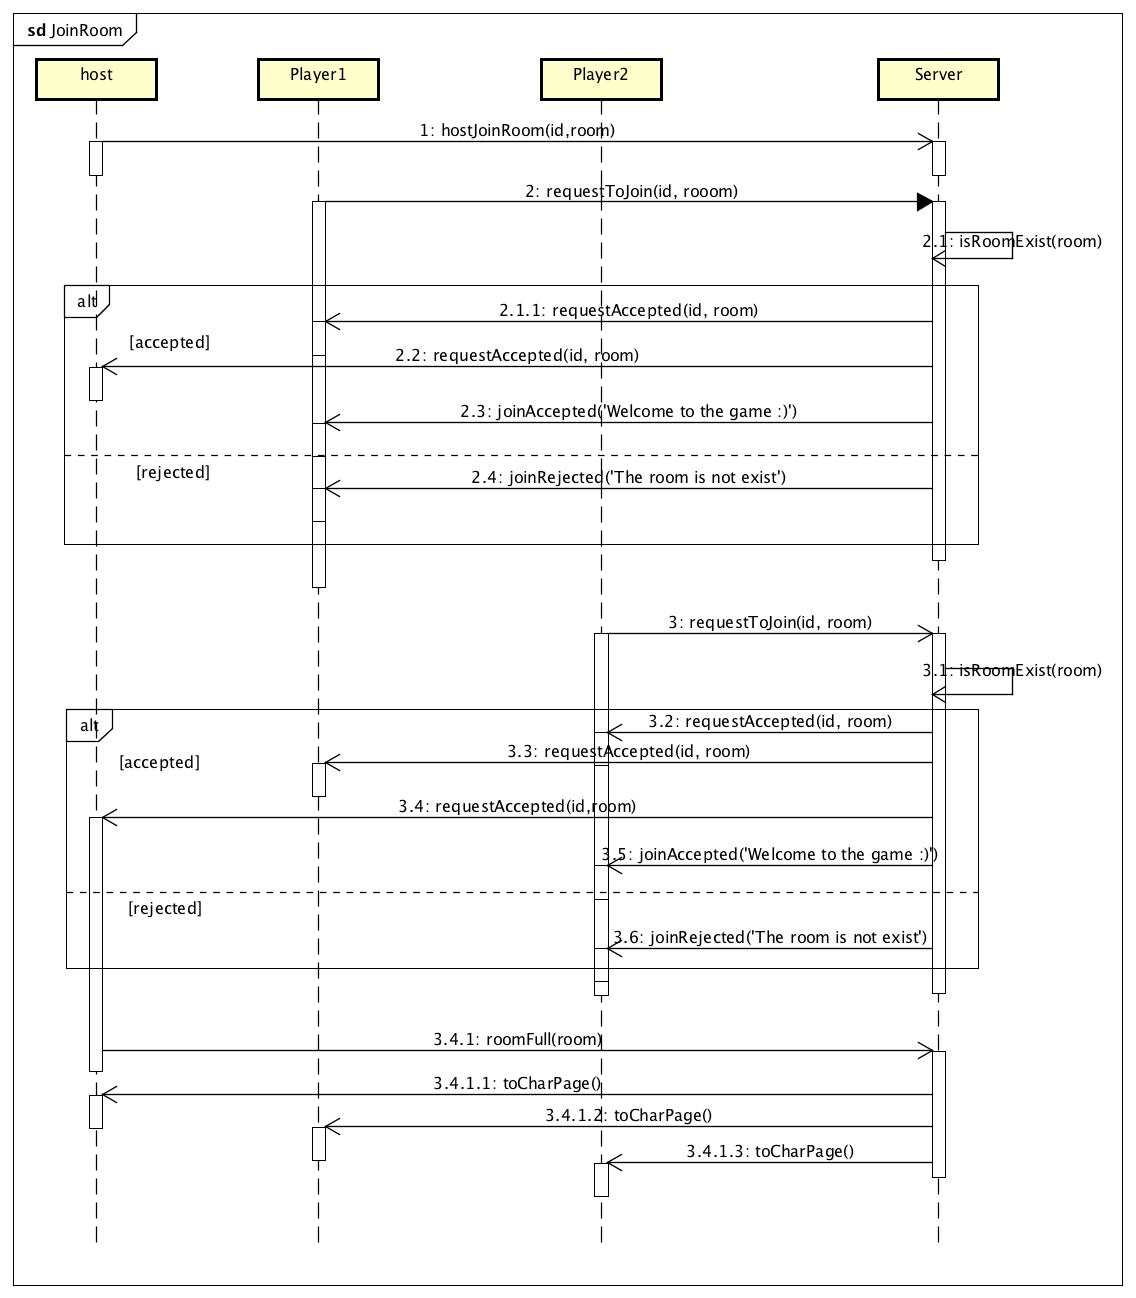
\includegraphics[scale=0.25]{Gambar/JoinRoom}
	\caption{Proses melakukan koneksi ke \textit{socket.io} dan bergabung kedalam \textit{room}.}
	\label{fig:1_JoinRoom}
\end{figure}

Pada awal permainan, \textit{client} pertama yang melakukan koneksi pada \textit{server} adalah \textit{PC}, yang berperan sebagai \textit{host} dalam permainan seperti yang dijelaskan pada Gambar \ref{fig:1_JoinRoom}.\textit{Host} akan menyediakan suatu kode yang berguna sebagai \textit{room} untuk kedua pemain yang akan bergabung dengan melakukan koneksi ke \textit{server}. \textit{Room} yang disediakan hanya akan menerima tiga \textit{client} saja, yaitu \textit{host}, \textit{player1}, dan \textit{player2}. 

\textit{Host} akan mengirimkan \textit{event} yang menandakan akan bergabung kedalam room, \textit{event} tersebut adalah \textbf{hostJoinRoom(id, room)}. \textit{Event} ini memiliki data yang akan dikirimkan kepada \textit{server}, data-data tersebut dijelaskan sebagai berikut:
\begin{itemize}
	\item \textbf{id}, identifikasi unik yang dimiliki masing-masing \textit{client} yang terkoneksi dengan Socket.io.
	\item \textbf{room}, suatu \textit{string} yang menandakan ruangan dimana \textit{client} hanya akan melakukan komunikasi didalam ruangan tersebut.
\end{itemize}

Data-data tersebut akan dikirimkan ke \textit{server} dan akan dimasukan kedalam suatu \textit{array} yang diproses oleh kelas \textit{Users}. Kelas ini memiliki \textit{array} dengan nama \textit{userArray} yang menyimpan seluruh \textit{client} yang telah terkoneksi dengan Socket.io. Kelas \textit{Users} akan bertanggung jawab dalam menyambung koneksi maupun memutus koneksi antara \textit{client} dan \textit{server}.

Setelah \textit{host} terkoneksi dengan Socket.io, maka \textit{room} milik \textit{host} sudah tersedia dan para pemain dapat bergabung kedalam \textit{room} tersebut. Untuk dapat mulai bermain, para pemain harus memasukan kode \textit{room} yang disediakan di halaman \textit{host} kedalah \textit{form} yang ada dihalaman \textit{browser} pada \textit{smartphone}. Pemain akan mengirimkan \textit{event} \textbf{requestToJoin(id, room)} pada \textit{server}. Data yang dikirimkan oleh pemain sama dengan data yang dikirimkan oleh \textit{host}. 

Setelah \textit{event} tersebut diterima oleh \textit{server}, maka akan dilakukan pengecekan apakah pemain dapat bergabung atau tidak kedalam \textit{room}. Pengecekan akan dilakukan didalam kelas \textit{Users}. Pengecekan tersebut dilakukan dengan menggunakan \textit{method} \textbf{isRoomExist(room)}. Beberapa pengecekan yang dilakukan \textit{method} ini akan dijelaskan sebagai berikut:
\begin{enumerate}
	\item Memeriksa apakah data \textit{room} didalam \textit{array} ada yang sesuai dengan parameter \textit{room}.
	\item Memeriksa apakah jumlah yang ada didalam \textit{room} yang dimaksud sudah lebih dari tiga atau belum.
\end{enumerate}

Apabila kedua hal diatas terpenuhi, maka pemain akan terkoneksi ke \textit{socket.io} dan bergabung ke dalam \textit{room}. \textit{Server} akan mengirimkan \textit{event} \textbf{requestAccepted(id, room)} kepada seluruh \textit{client} yang berada di \textit{room} tersebut. \textit{Event} tersebut akan ditangkap oleh \textit{host} yang berfungsi untuk mencatat sudah ada berapa pemain yang berhasil masuk kedalam \textit{room}. \textit{Server} pun akan mengirimkan \textit{event} \textbf{joinAccepted('Welcome to the game :)')} kepada pemain yang berhasil bergabung kedalam \textit{room}. \textit{Event} tersebut berfungsi untuk memberikan \textit{feedback} kepada pemain bahwa pemain telah berhasil bergabung kedalam permainan.

Apabila kedua hal diatas tidak terpenuhi, maka pemain tidak dapat terkoneksi ke Socket.io. \textit{Server} akan mengirimkan \textit{event} \textbf{joinRejected('The room is not exist')} kepada pemain. \textit{Event} tersebut berfungsi sebagai \textit{feedback} kepada pemain yang tidak dapat bergabung. Pemain pertama yang berhasil bergabung akan berperan sebagai \textit{Player1}. Setelah satu pemain bergabung, maka \textit{server} akan menunggu untuk pemain kedua agar permainan dapat dimulai. Pemain kedua akan melakukan hal yang sama dengan pemain pertama untuk dapat bergabung kedalam room.

Setelah \textit{room} berisi tiga \textit{client}, maka \textit{host} akan mengirimkan \textit{event} \textbf{roomFull(room)} kepada \textit{server}. \textit{Event} tersebut menandakan bahwa \textit{room} sudah tidak dapat menerima \textit{client} yang akan bergabung. Setelah \textit{event} tersebut diterima oleh \textit{server}, maka \textit{event} \textbf{toCharPage()} akan dipancarkan oleh \textit{server} kepada seluruh \textit{client} yang ada didalam \textit{room} tersebut. \textit{Event} ini berfungsi untuk mengganti halaman saat ini ke halaman selanjutnya.

\subsection{\textit{Sequence} Memilih Karakter}

\begin{figure}[H]
	\centering
	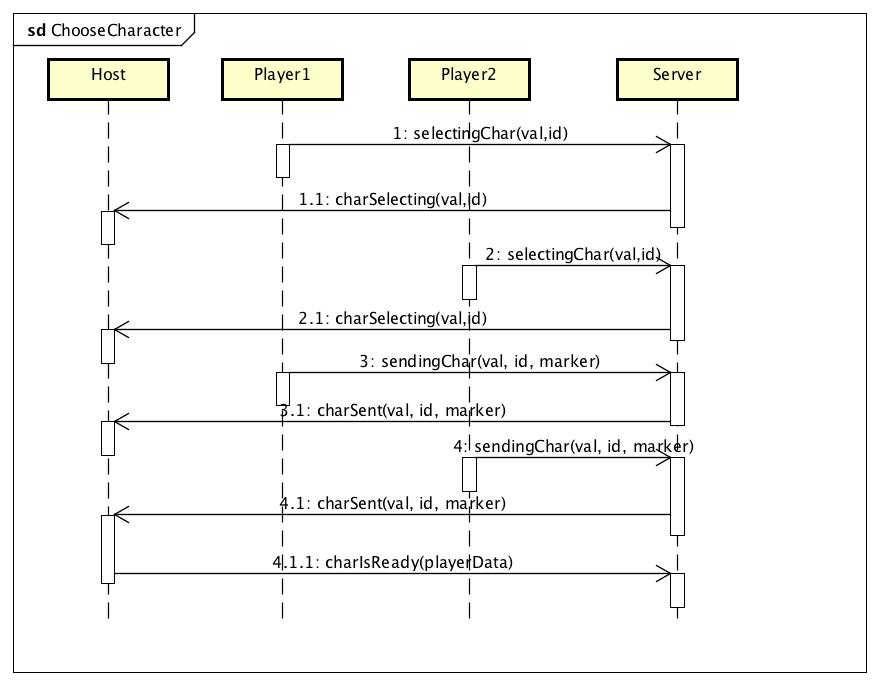
\includegraphics[scale=0.35]{Gambar/ChooseCharacter}
	\caption{Proses memilih karakter.}
	\label{fig:2_ChooseCharacter}
\end{figure}

Halaman ini merupakan halaman yang dituju oleh para pemain yang telah berhasil melakukan koneksi dan bergabung kedalam \textit{room}. Para pemain akan memilih karakter yang ada dihalaman \textit{browser} pada \textit{smartphone}, dimana karakter yang dipilih akan muncul dihalaman \textit{browser} pada \textit{PC}.Seperti yang dijelaskan pada Gambar \ref{fig:2_ChooseCharacter}, pemain yang memilih karakter tertentu akan mengirimkan \textit{event} \textbf{selectingChar(val, id)} kepada \textit{server}. Data-data yang dikirimkan akan dijelaskan sebagai berikut:
\begin{itemize}
	\item \textbf{val}, identifikasi unik yang dimiliki oleh masing-masing karakter.
	\item \textbf{id}, identifikasi unik yang dimiliki masing-masing \textit{client} yang terkoneksi dengan Socket.io.
\end{itemize}
Setelah \textit{event} tersebut diterima oleh \textit{server}, maka server akan mengirimkan \textit{event} \textbf{charSelecting(val, id)} kepada \textit{host}. \textit{Event} tersebut berfungsi untuk menampilkan karakter yang dipilih oleh pemain dihalaman \textit{PC}.

Apabila pemain akan menetapkan karakter yang telah ditampilkan dihalaman \textit{PC}, maka \textit{pemain} akan mengirimkan \textit{event} \textbf{sendingChar(val,id,marker)} kepada \textit{server}. Data-data tersebut sama seperti yang dikirimkan oleh \textit{event} sebelumnya, hanya saja ada tambahan data \textbf{marker} pada parameter. Data tambahan tersebut berfungsi sebagai penanda bahwa sudah ada satu pemain yang telah menetapkan karakter yang akan dimainkan. Setelah \textit{server} menerima \textit{event} tersebut, maka \textit{server} akan meneruskan data-data yang sudah diterima pada \textit{host} dengan mengirimkan \textit{event} \textbf{charSent(val,id,marker)}. Apabila \textit{event} tersebut telah diterima oleh \textit{host}, maka karakter telah dimiliki oleh pemain yang menetapkannya.

Pemain kedua pun akan melakukan hal yang sama untuk memilih dan menetapkan karakter yang akan dimainkan. Apabila kedua pemain telah menetapkan karakter yang akan dimainkan, \textit{host} akan memancarkan \textit{event} \textbf{charIsReady(playerData)}.Data yang dikirimkan merupakan suatu objek \textit{array} yang berisi data para pemain dan data karakter yang telah dipilih.\textit{Event} tersebut berfungsi untuk memberi informasi kepada \textit{server} untuk pindah kehalaman selanjutnya.

\subsection{\textit{Sequence} Memulai Permainan}

\begin{figure}[H]
	\centering
	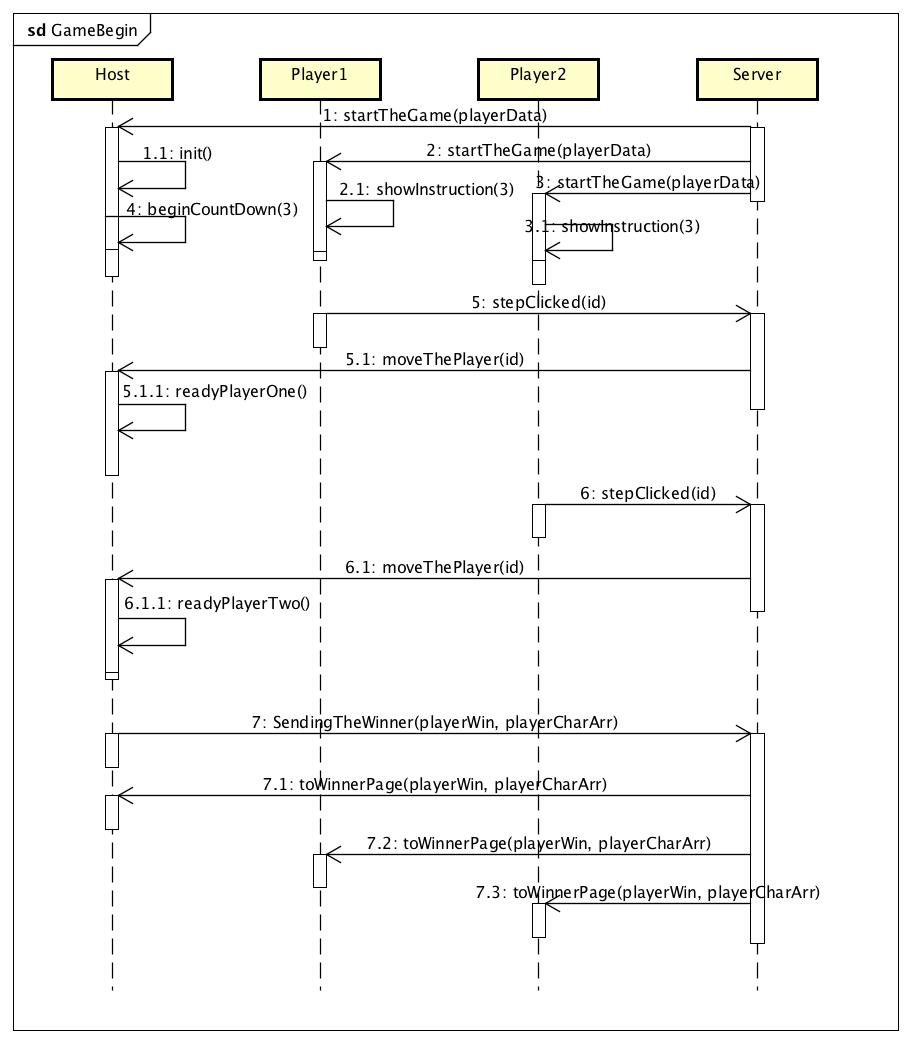
\includegraphics[scale=0.33]{Gambar/GameBegin}
	\caption{Proses memulai permainan.}
	\label{fig:3_GameBegin}
\end{figure}

Pada tahap ini, \textit{server} akan memancarkan \textit{event} \textbf{startTheGame(playerData)}. Seperti yang dijelaskan pada Gambar \ref{fig:3_GameBegin}, data yang dikirimkan merupakan data yang didapatkan dari \textit{event} sebelumnya. \textit{Event} tersebut akan diterima oleh seluruh \textit{client} yang berada didalam \textit{room} tertentu, yang kemudian akan memulai permainannya. \textit{Host} akan mengeksekusi \textit{method} \textbf{init()} dan \textbf{beginCountDown(3)} untuk memulai permainan. \textit{Method} \textbf{init()} berfungsi untuk mulai menggambar lintasan lari di halaman \textit{PC} yang akan menjadi tempat para karakter dimainkan. \textit{Method} \textbf{beginCountDown(3)} berfungsi untuk melakukan hitungan mundur selama tiga detik sebelum permainan dapat dimulai. 

Para pemain yang menerima \textit{event} \textbf{startTheGame(playerData)} akan mengeksekusi \textit{method} \textbf{showInstruction(3)}. \textit{Method} tersebut berfungsi untuk menampilkan instruksi untuk memainkan permainan selama tiga detik. Apabila hitungan mundur telah selesai, maka permainan akan dimulai.

Permainan dilakukan dengan cara menekan tombol-tombol yang ada pada halaman \textit{smartphone}. Apabila pemain menekan tombol, maka \textit{event} \textbf{stepClicked(id)} akan dipancarkan. \textit{Server} akan menerima \textit{event} tersebut, yang kemudian akan meneruskannya dengan memancarkan \textit{event} \textbf{moveThePlayer(id)} kepada \textit{host}. Setelah \textit{event} tersebut diterima oleh \textit{host}, maka \textit{host} akan menjalankan \textit{method} tertentu untuk menggerakan karakter milik pemain. Apabila \textit{Player1} yang menekan tombol, maka \textit{method} \textbf{readyPlayerOne()} akan dieksekusi oleh \textit{host}. Apabila \textit{Player2}, maka \textbf{readyPlayerTwo()} akan dieksekusi. Kedua \textit{Method} tersebut berfungsi untuk memindahkan posisi karakter milik pemain dari posisi semula hingga posisi tertentu. Permainan akan berakhir apabila ada karakter yang menyentuh garis akhir pertama kali.

Apabila ada pemain yang berhasil menyentuh garis akhir, maka \textit{host} akan memancarkan \textit{event} \textbf{sendingTheWinner(playerWin, playerCharArr)}. Data-data yang dikirimkan akan dijelaskan sebagai berikut:
\begin{itemize}
	\item \textbf{playerWin}, angka \textit{integer} yang menandakan pemain nomor berapa yang memenangkan permainan.
	\item \textbf{playerCharArr}, \textit{array} yang menyimpan karakter dari masing-masing pemain.
\end{itemize}
\textit{Server} akan menangkap \textit{event} tersebut dan meneruskannya dengan memancarkan \textit{event} \textbf{toWinnerPage(playerWin, playerCharArr)} ke setiap \textit{client} pada \textit{room} tertentu. \textit{Event} tersebut berfungsi untuk berpindah ke halaman selanjutnya.

\subsection{\textit{Sequence} Mengakhiri Permainan}
\begin{figure}[H]
	\centering
	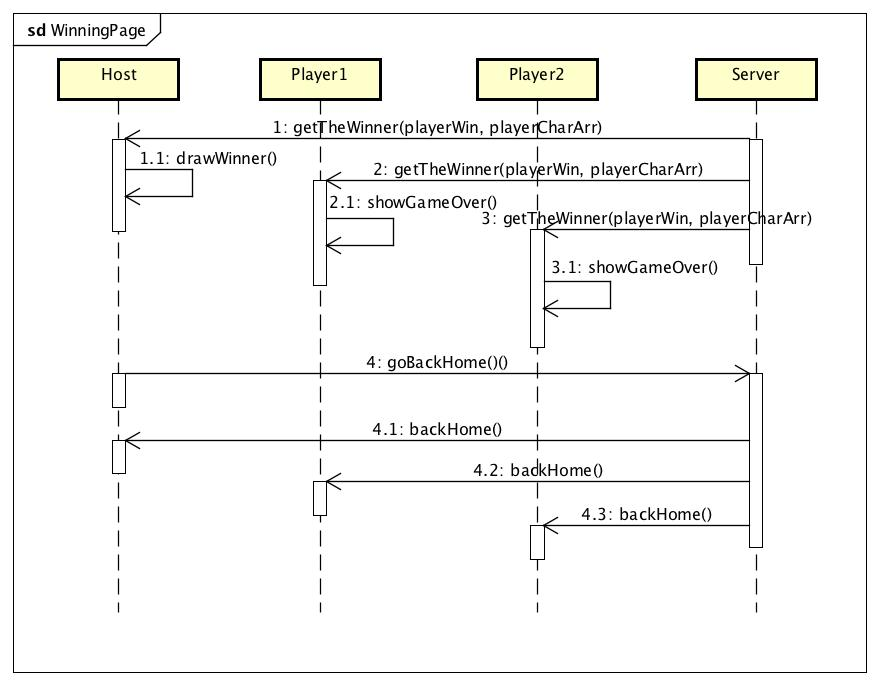
\includegraphics[scale=0.33]{Gambar/WinningPage}
	\caption{Menampilkan para pemain yang telah selesai bermain.}
	\label{fig:4_WinningPage}
\end{figure}

Pada tahap ini, \textit{server} akan memancarkan \textit{event} \textbf{getTheWinner(playerWin, playerCharArr)} dengan data-data yang diterima dari \textit{event} sebelumnya. Seperti yang dijelaskan pada Gambar \ref{fig:4_WinningPage} \textit{host} akan menerima \textit{event} tersebut dan akan mengeksekusi \textit{method} \textbf{drawWinner()}. \textit{Method} tersebut berfungsi untuk menampilkan karakter milik para pemenang yang telah selesai bermain. Para pemain akan menerima \textit{event} yang dipancarkan oleh \textit{server} dan mengeksekusi \textit{method} \textbf{showGameOver()}. \textit{Method} ini akan menampilkan teks yang menunjukan bahwa permainan telah selesai.

Apabila pemain menekan tombol \textit{exit} yang ada dihalaman \textit{browser} pada \textit{PC}, maka \textit{host} akan memancarkan \textit{event} \textbf{goBackHome()}. \textit{Event} tersebut akan diterima oleh \textit{server} dan akan diteruskan dengan memancarkan \textit{event} \textbf{backHome()}. Seluruh \textit{client} didalam \textit{room} yang menerima \textit{event} tersebut akan kembali kehalaman utama dan koneksi Socket.io pun akan terputus.


\section{Perancangan Antarmuka}
\label{sec:antarmuka}

Antarmuka yang dirancang terbagi menjadi dua bagian, yaitu antarmuka yang ada di \textit{PC} dan \textit{smartphone}.

\begin{enumerate}
	\item Antarmuka halaman utama
	
	\textbf{PC}
	
	Halaman ini merupakan halaman utama yang pertama kali dituju oleh pengguna yang menggunakan \textit{PC}. Komponen halaman ini terdiri dari dua buah gambar jari yang melambangkan permainan, teks yang menunjukan nama permainan yaitu \textit{finger for life}, dan tombol \textit{start} yang digunakan untuk memulai permainan. Rancangan antarmuka halaman \textit{home} dapat dilihat pada Gambar \ref{fig:web1_home}

\begin{figure}[H]
	\centering
	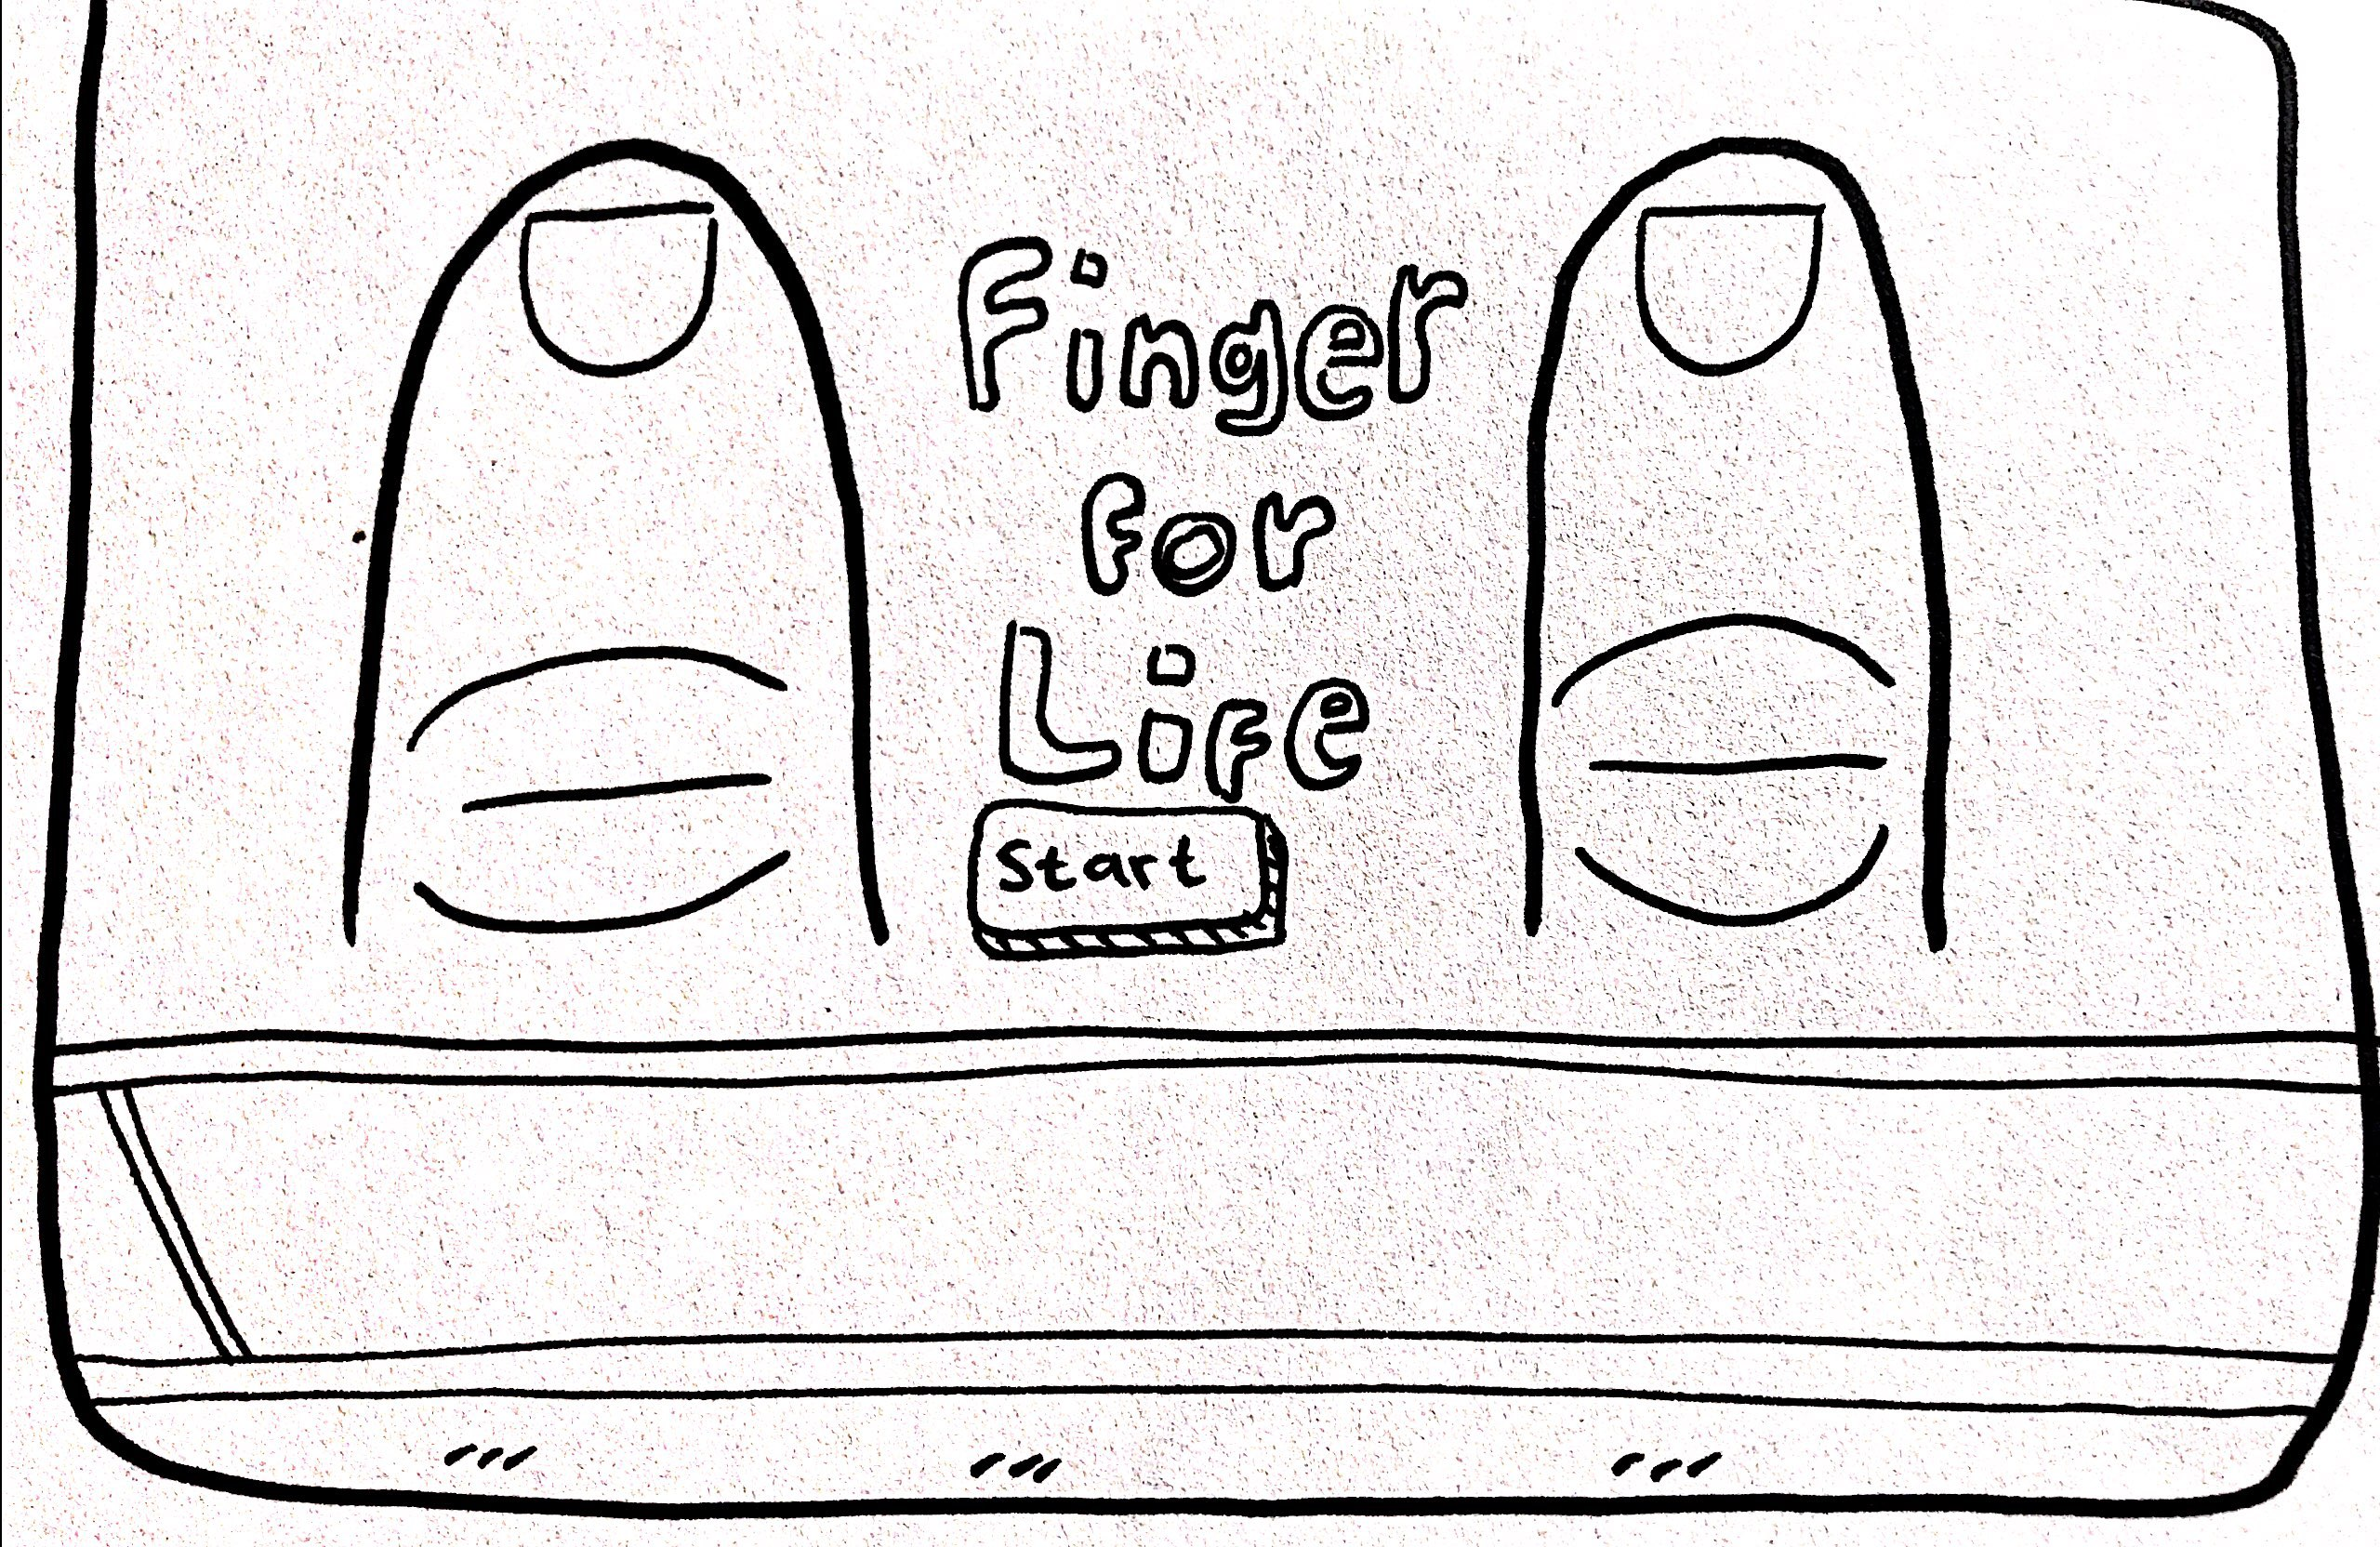
\includegraphics[scale=0.1]{Gambar/web1_home}
	\caption{Halaman pada \textit{PC} yang menunjukan halaman utama saat \textit{client} mengakses alamat web.}
	\label{fig:web1_home}
\end{figure}

	\textbf{Smartphone}
	
	Halaman ini merupakan halaman utama yang pertama kali dituju oleh pengguna yang menggunakan \textit{smartphone}. Komponen halaman ini terdiri dari teks yang menunjukan nama permainan yaitu \textit{finger for life}, dan tombol \textit{join} yang digunakan untuk memulai permainan. Rancangan antarmuka halaman \textit{home} dapat dilihat pada Gambar \ref{fig:mob1_home}.
	
\begin{figure}[H]
	\centering
	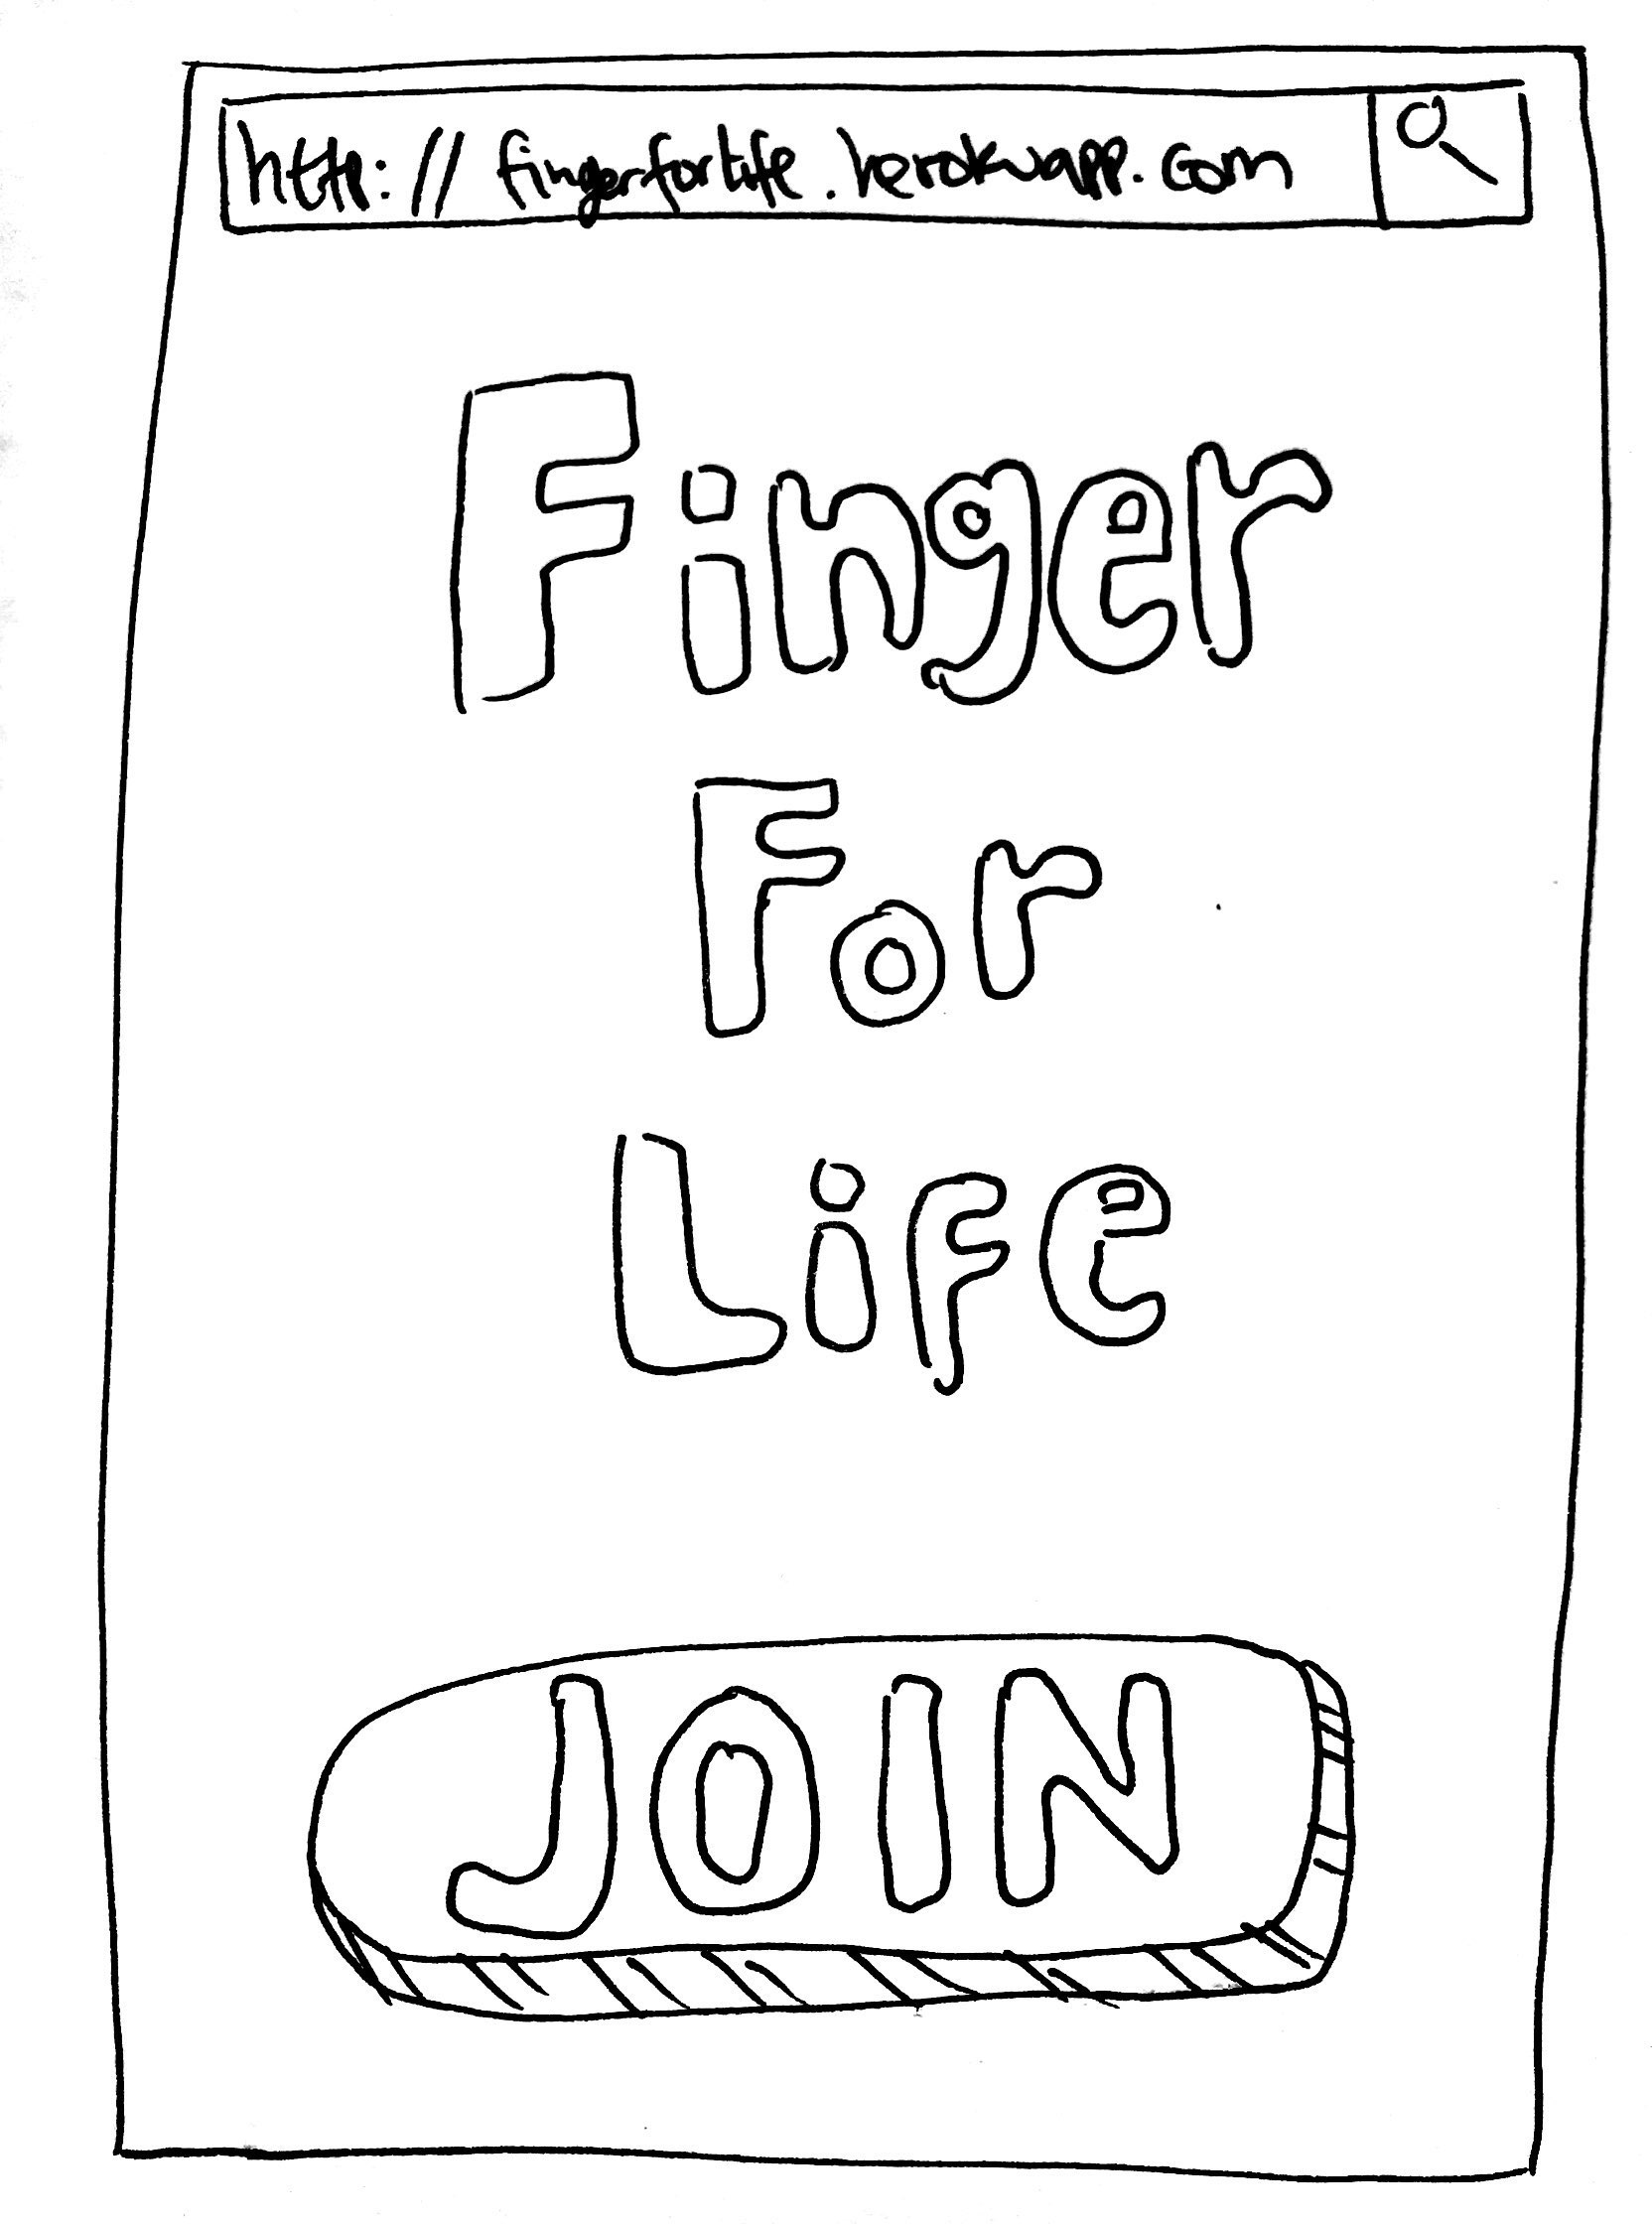
\includegraphics[scale=0.1]{Gambar/mob1_home}
	\caption{Halaman pada \textit{mobile} yang menunjukan halaman utama saat \textit{client} mengakses alamat web.}
	\label{fig:mob1_home}
\end{figure}

	\item Antarmuka halaman Permintaan Bergabung
	
	\textbf{PC}
	
	Halaman ini menampilkan suatu perintah yang dapat dilakukan oleh pengguna apabila akan bergabung kedalam permainan. Halaman ini pun menyediakan suatu kode untuk para pemain dimana kode tersebut akan berfungsi sebagai suatu \textit{room} bagi para pemain. Pada halaman ini akan dilakukan proses sinkronisasi untuk para pengguna, apakah berhasil bergabung dalam permainan atau tidak. Apabila berhasil, maka akan muncul suatu teks yang menunjukan suatu pemain telah berhasil bergabung. Apabila tidak, maka tidak akan menampilkan apapun dan halaman tidak akan menuju ke halaman selanjutnya sebelum ada dua pemain yang berhasil bergabung. Rancangan antarmuka halaman permintaan bergabung pada \textit{PC} dapat dilihat pada Gambar \ref{fig:web2_sync}.
	
\begin{figure}[H]
	\centering
	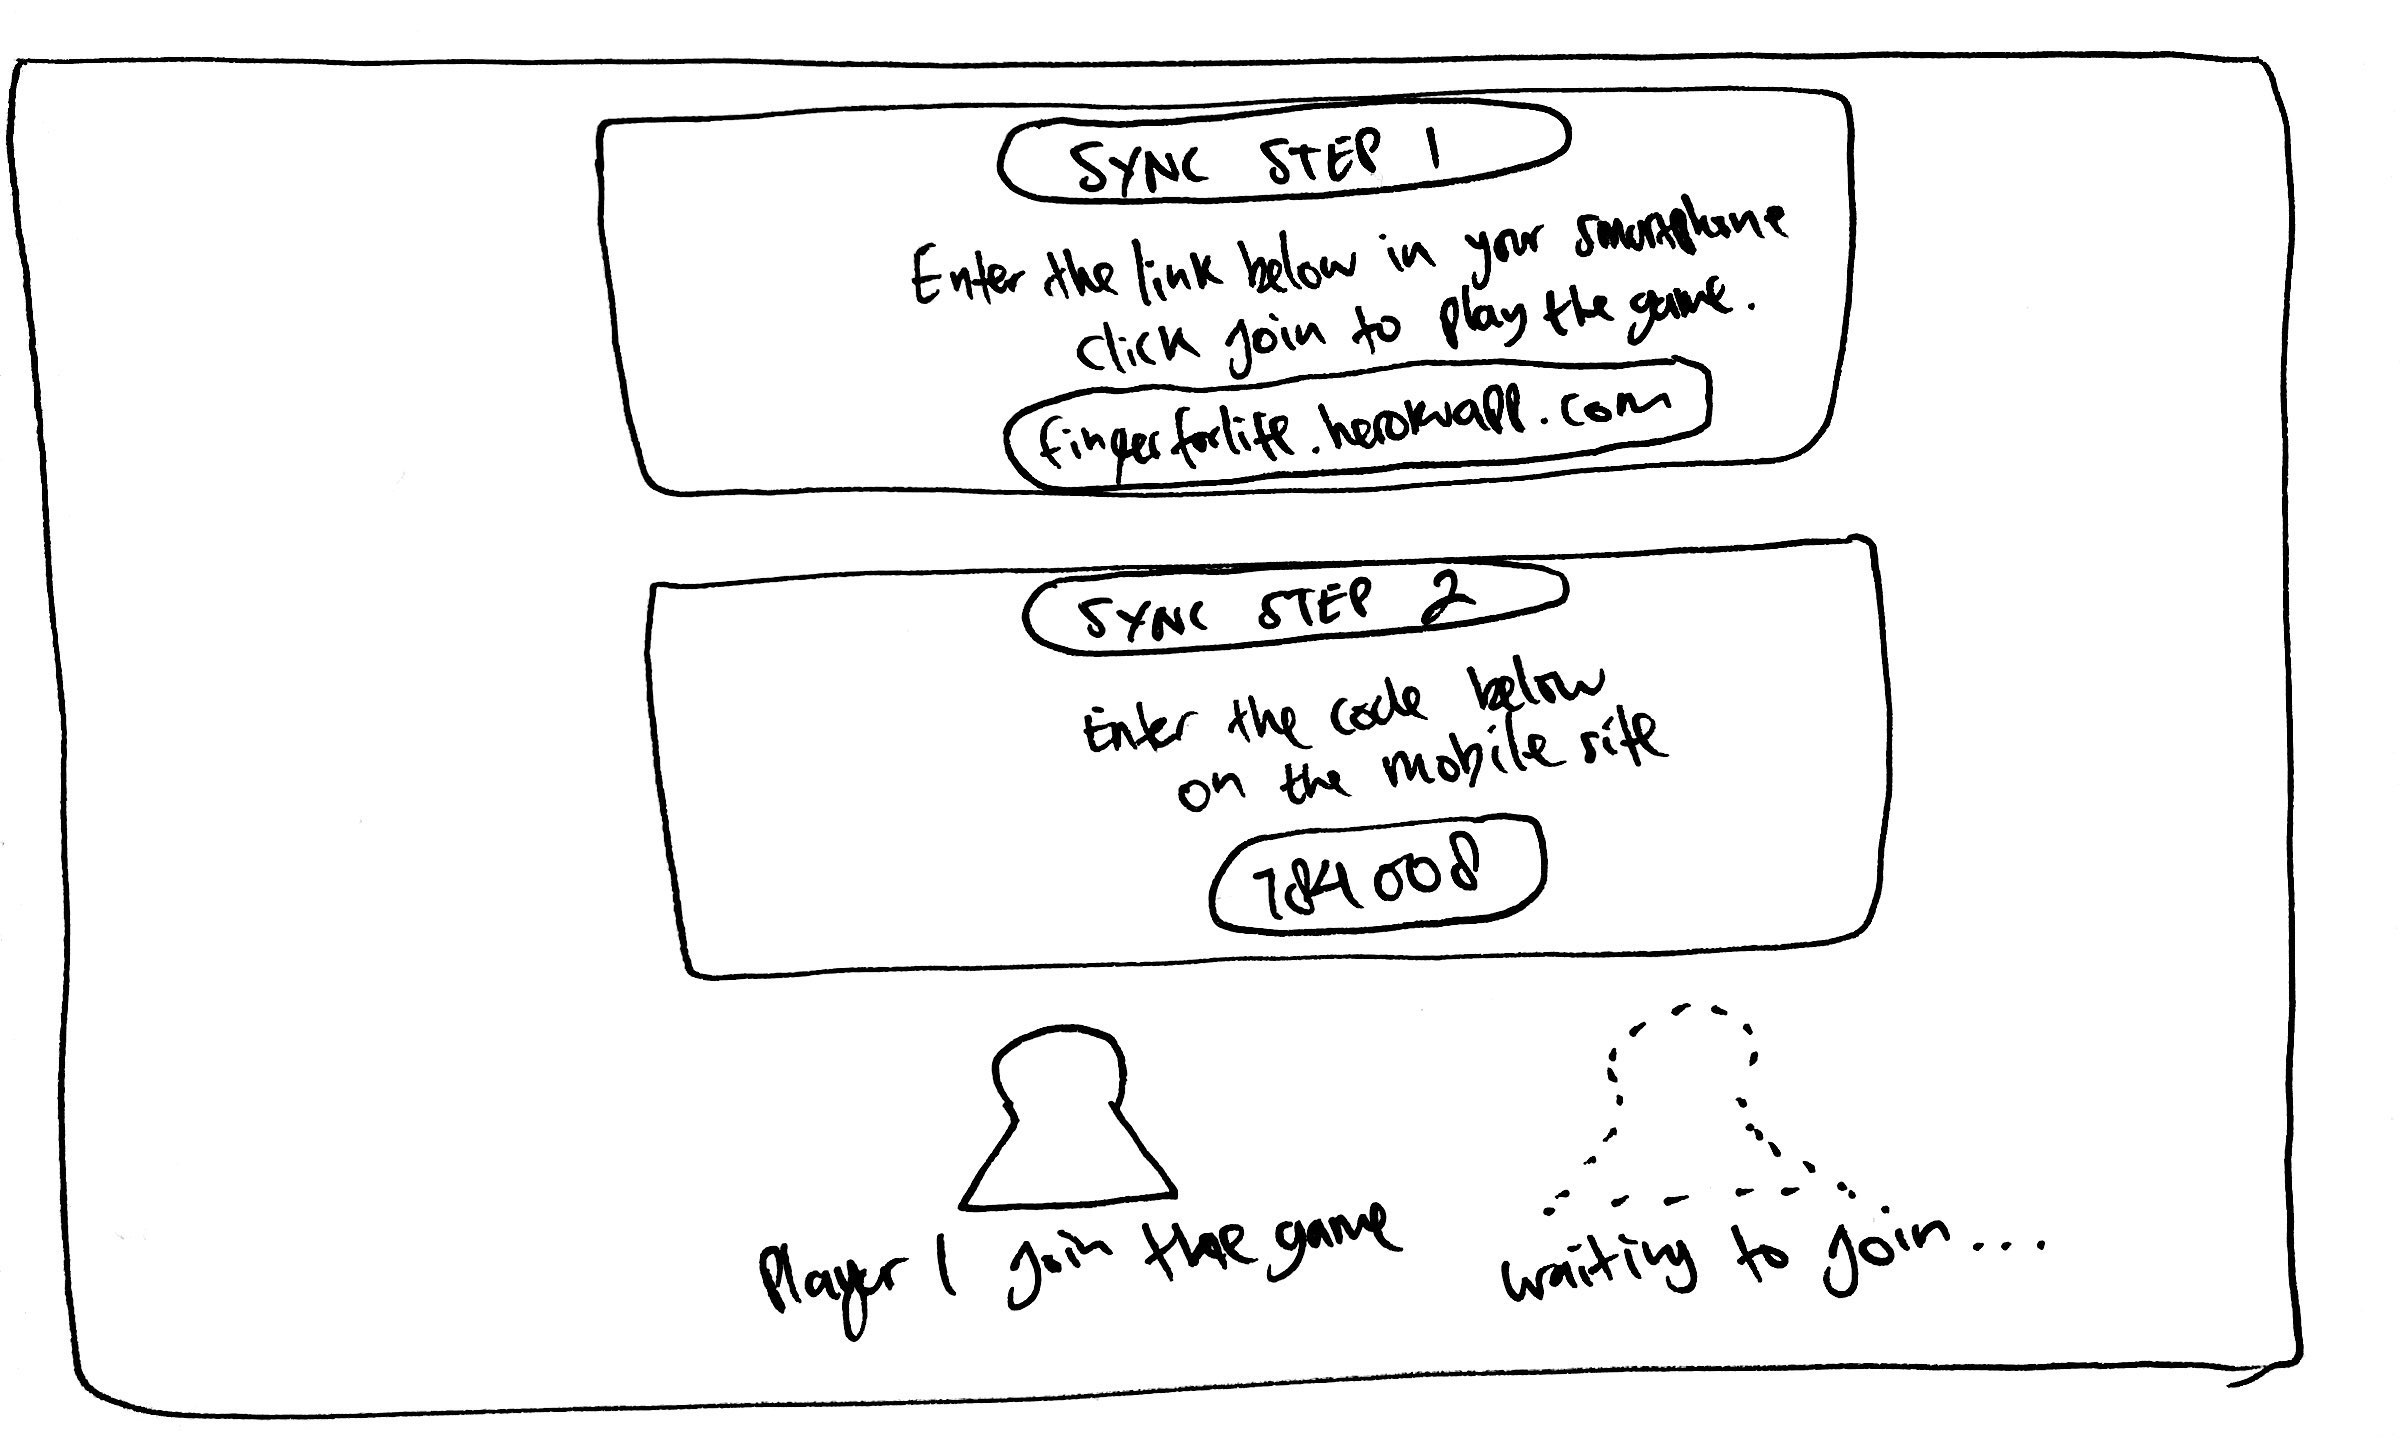
\includegraphics[scale=0.1]{Gambar/web2_sync}
	\caption{Halaman pada \textit{PC} yang menampilkan langkah untuk bergabung kedalam permainan}
	\label{fig:web2_sync}
\end{figure}

	\textbf{Smartphone}
	
	Halaman ini berfungsi untuk melakukan permintaan untuk bergabung kedalam permainan. Komponen halaman ini terdiri dari kolom kode, dan tombol \textit{send}. \textit{client} harus mengisi kode yang disediakan dihalaman \textit{PC} kedalam kolom kode. Setelah mengisi kode, maka \textit{client} harus menekan tombol \textit{send} untuk mengirim kode tersebut kepada \textit{server} untuk dilakukan pengecekan. Rancangan antarmuka halaman permintaan bergabung pada \textit{smartphone} dapat dilihat pada Gambar \ref{fig:mob2_sync1}.
	
\begin{figure}[H]
	\centering
	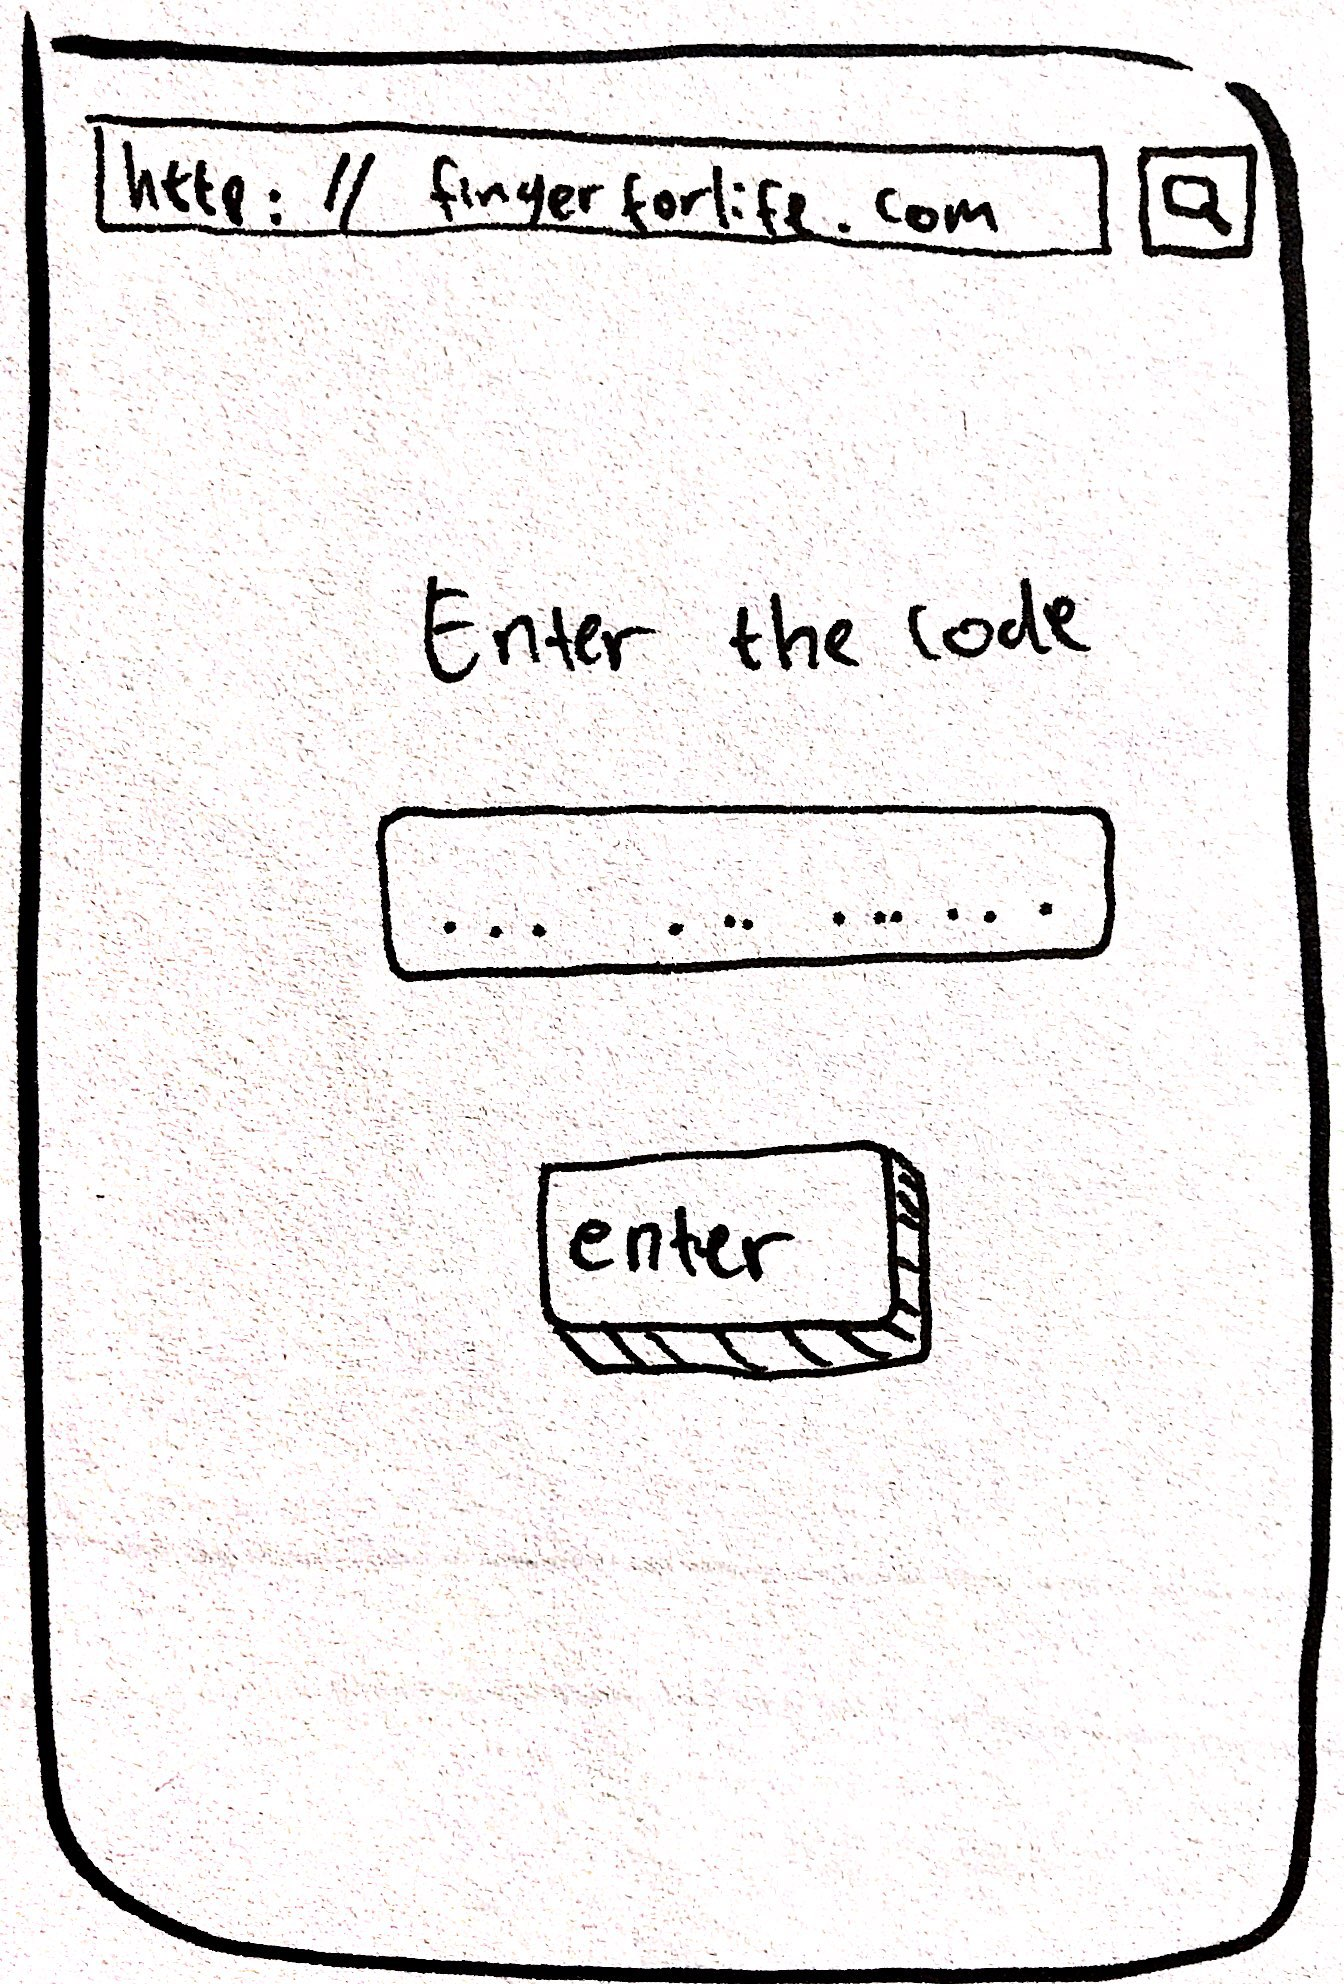
\includegraphics[scale=0.1]{Gambar/mob2_sync1}
	\caption{Halaman pada \textit{smartphone} yang menampilkan kolom untuk mengisi kode.}
	\label{fig:mob2_sync1}
\end{figure}

\item Antarmuka halaman Memilih Karakter

	\textbf{PC}
	
	Halaman ini akan menampilkan karakter yang telah dipilih oleh pemain. Apabila karakter belum memilih karakter yang akan dimainkan, maka halaman ini belum menampilkan apapun. Rancangan antarmuka halaman memilih karakter pada \textit{PC} dapat dilihat pada Gambar \ref{fig:web3_char}.
	
\begin{figure}[H]
	\centering
	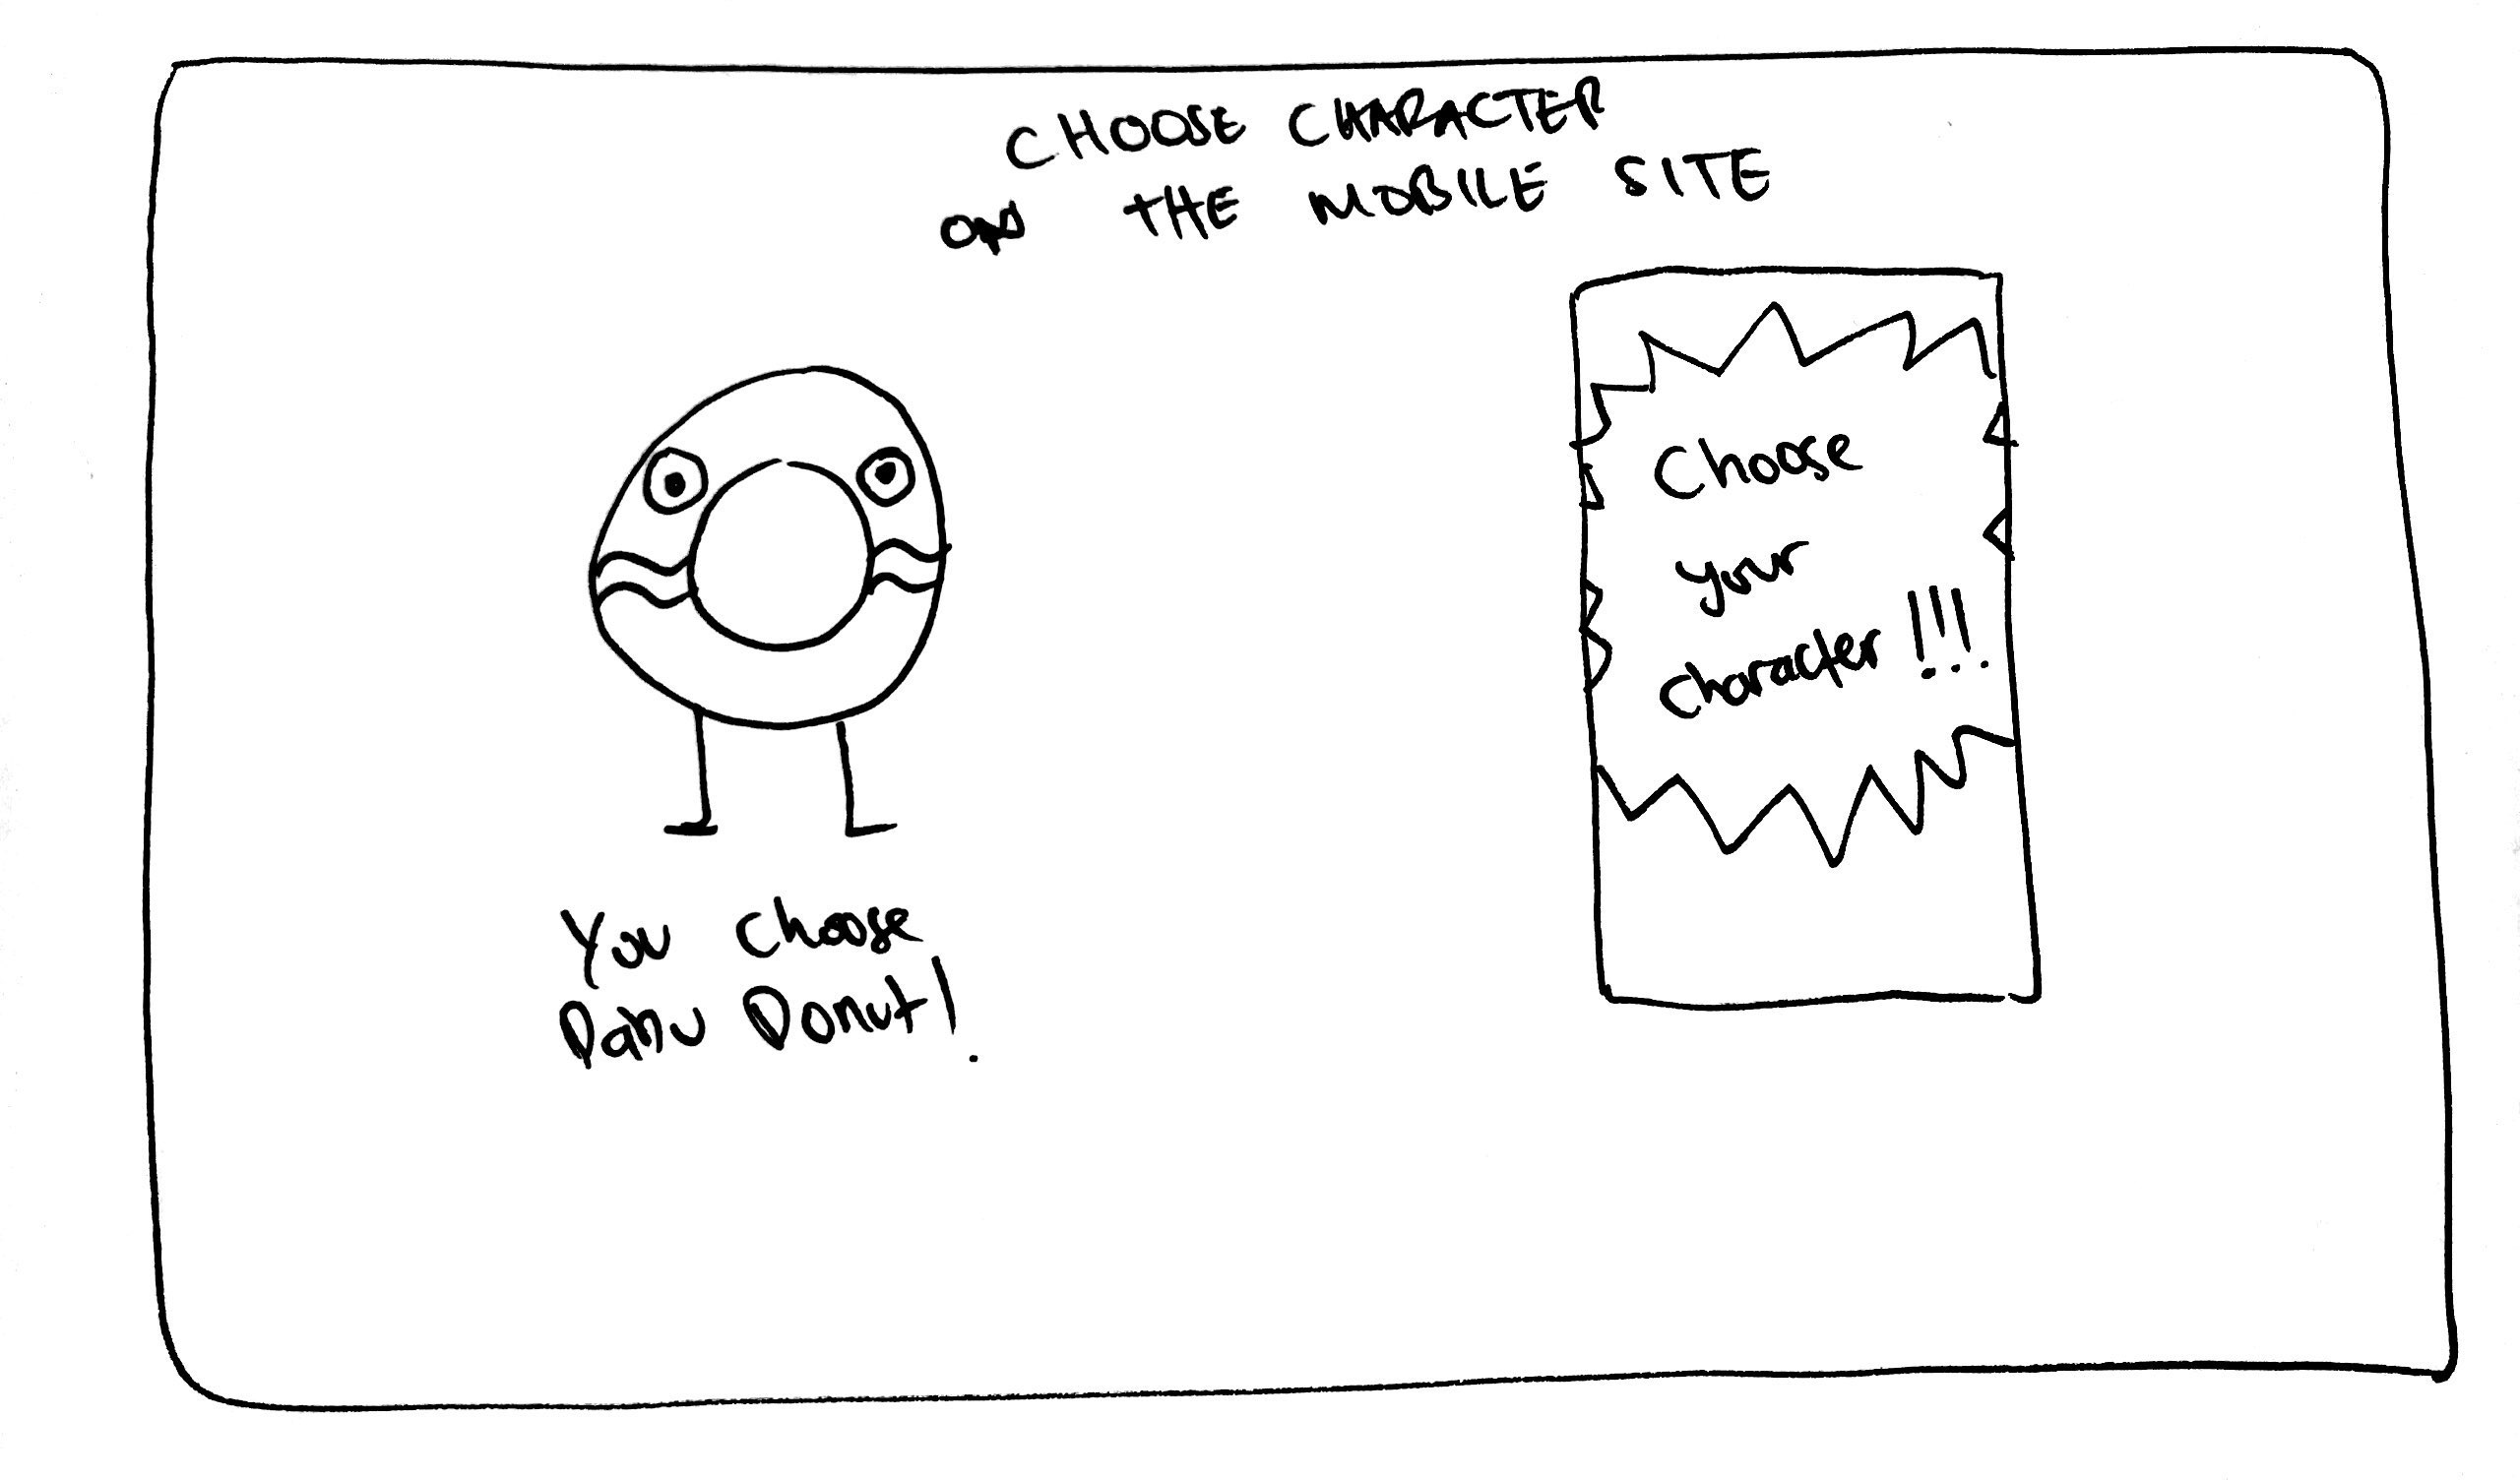
\includegraphics[scale=0.1]{Gambar/web3_char}
	\caption{Halaman pada \textit{PC} yang menampilkan karakter yang telah ditetapkan oleh pemain.}
	\label{fig:web3_char}
\end{figure}


	\textbf{Smartphone}
	
	Halaman ini akan menampilkan daftar karakter yang dapat dimainkan oleh pemain. Komponen halaman ini terdiri dari daftar karakter, dan tombol \textit{choose}. Rancangan antarmuka halaman memilih karakter pada \textit{smartphone} dapat dilihat pada Gambar \ref{fig:mob3_char1}.
	
\begin{figure}[H]
	\centering
	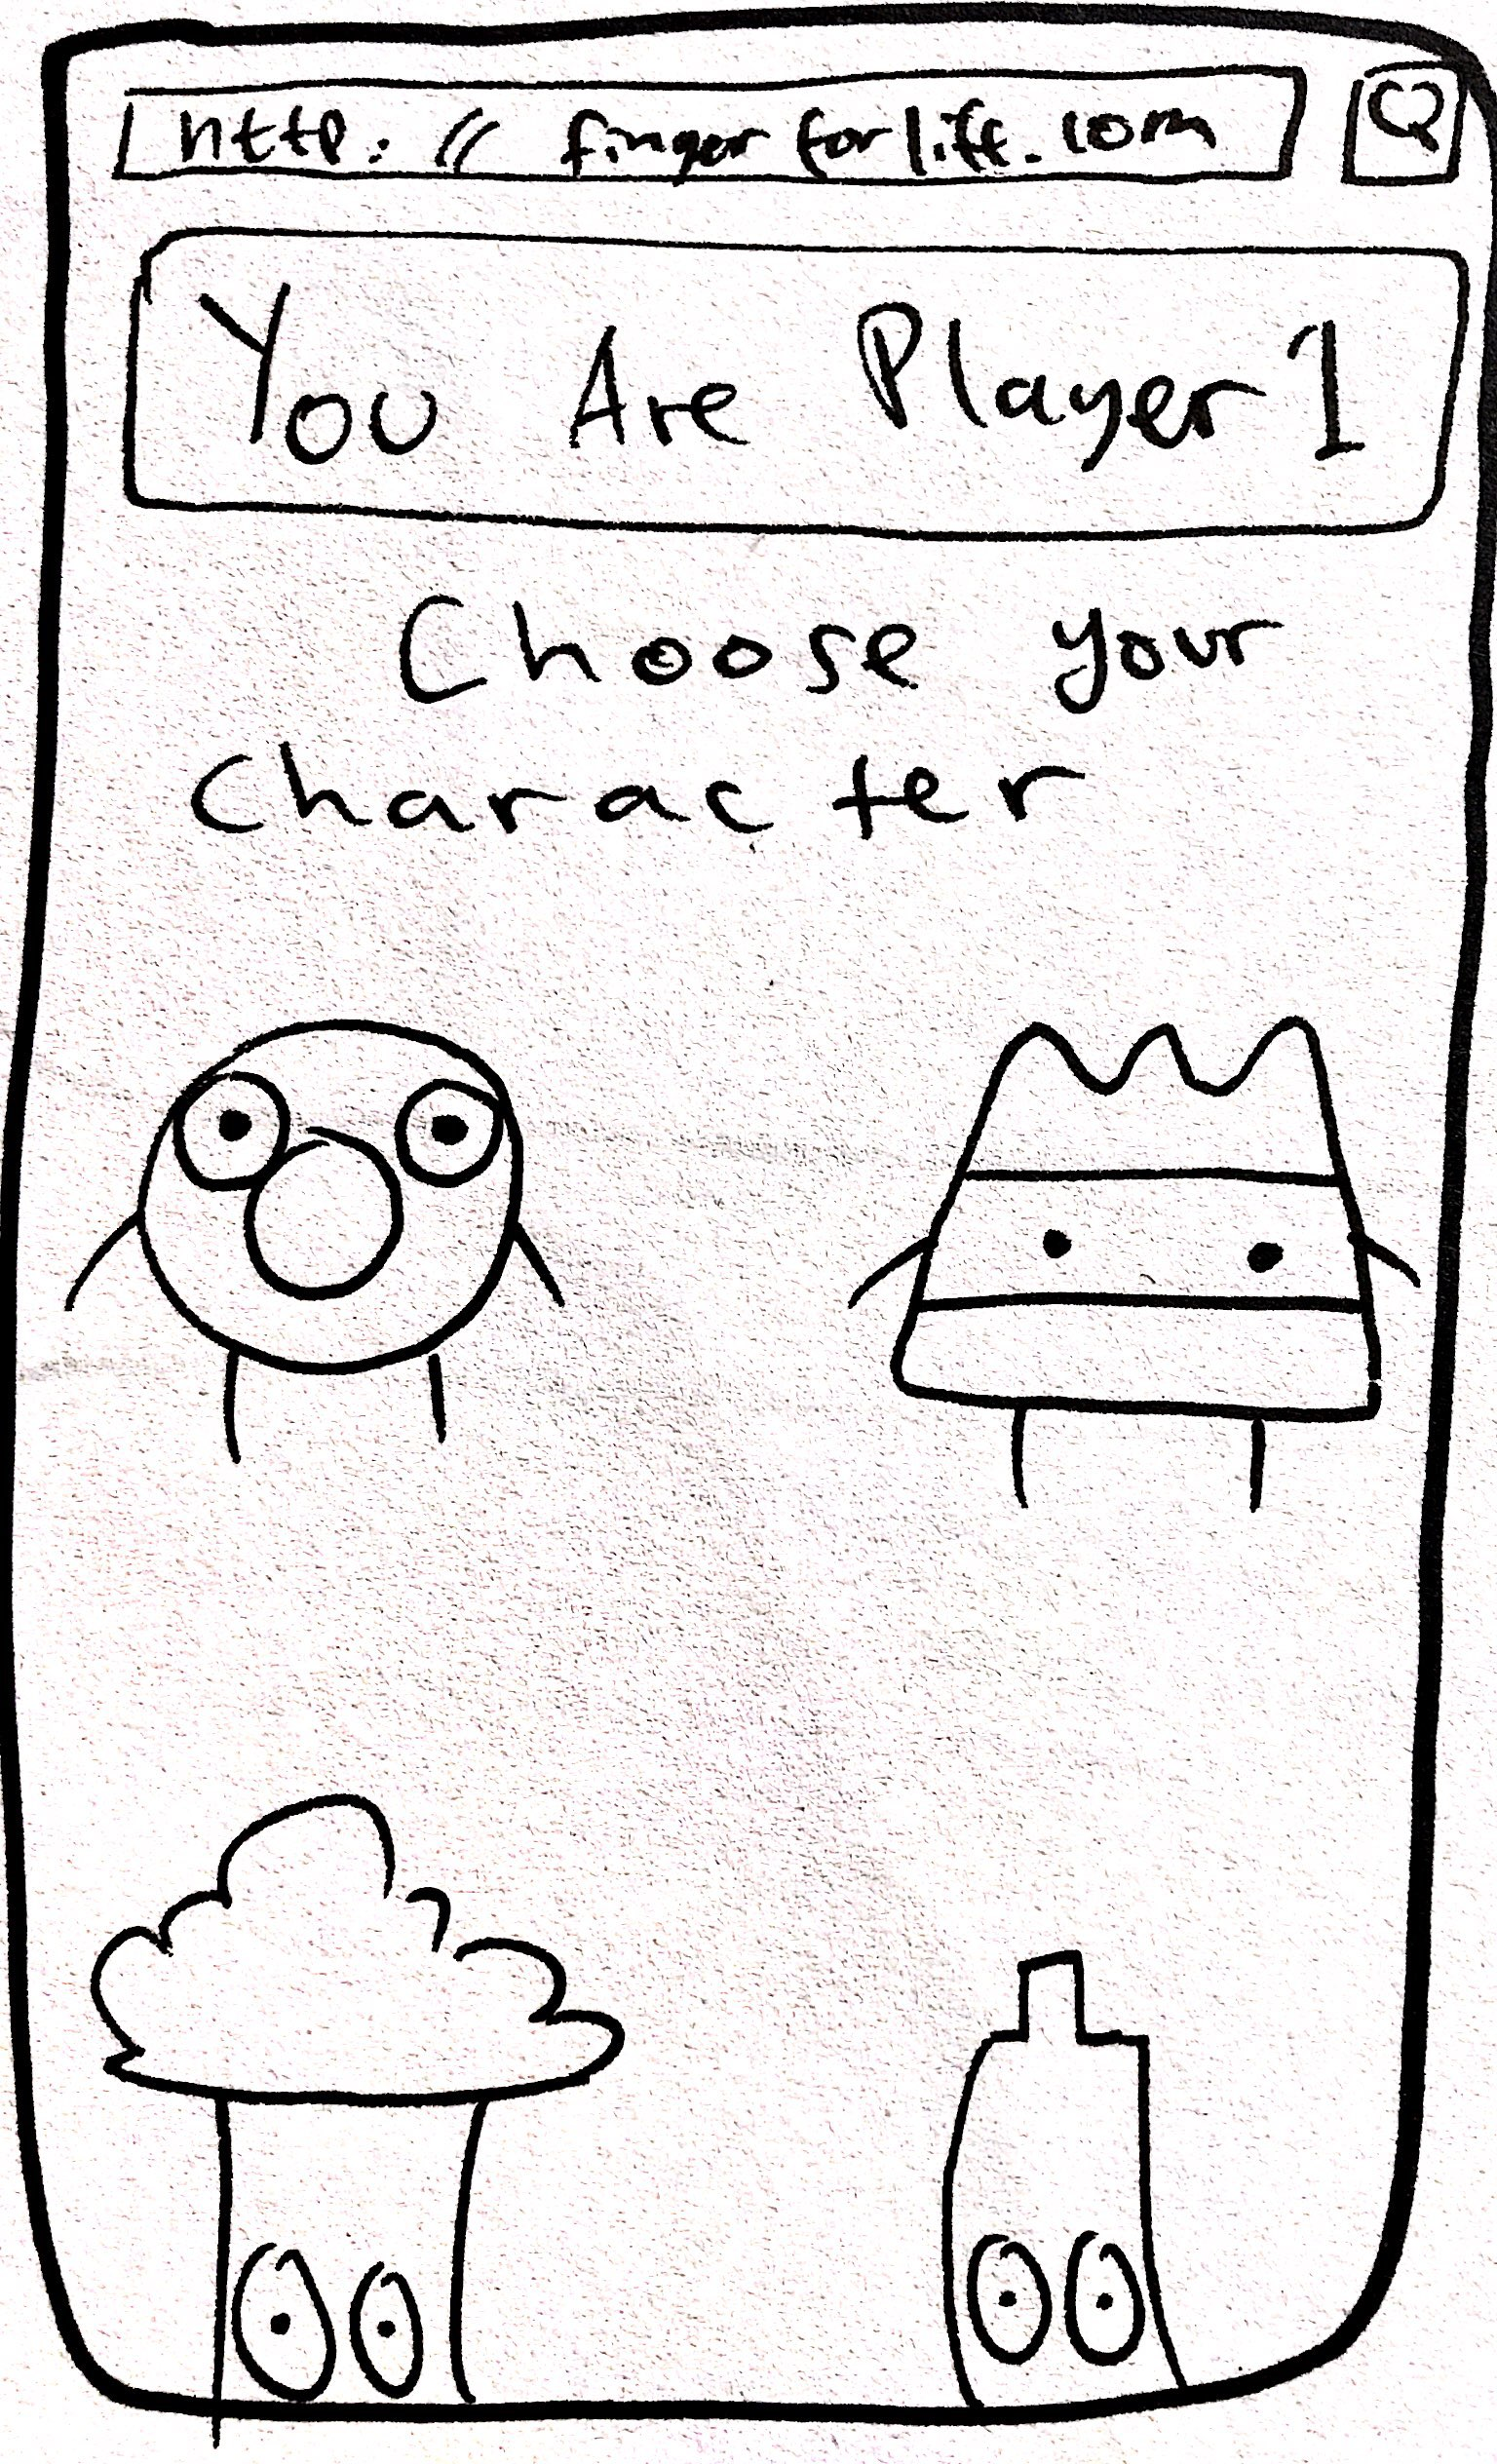
\includegraphics[scale=0.1]{Gambar/mob3_char1}
	\caption{Halaman pada \textit{smartphone} yang menampilkan daftar karakter yang dapat dipilih.}
	\label{fig:mob3_char1}
\end{figure}

\item Antarmuka halaman Memulai permainan

	\textbf{PC}
	
	Halaman ini menampilkan arena permainan untuk para pemain. Komponen halaman ini terdiri dari suatu gambar lintasan lari, dan karakter yang telah dipilih pada halaman sebelumnya. Rancangan antarmuka halaman \textit{gameplay} pada \textit{PC} dapat dilihat pada Gambar \ref{fig:web5_gameplay2}.
	
\begin{figure}[H]
	\centering
	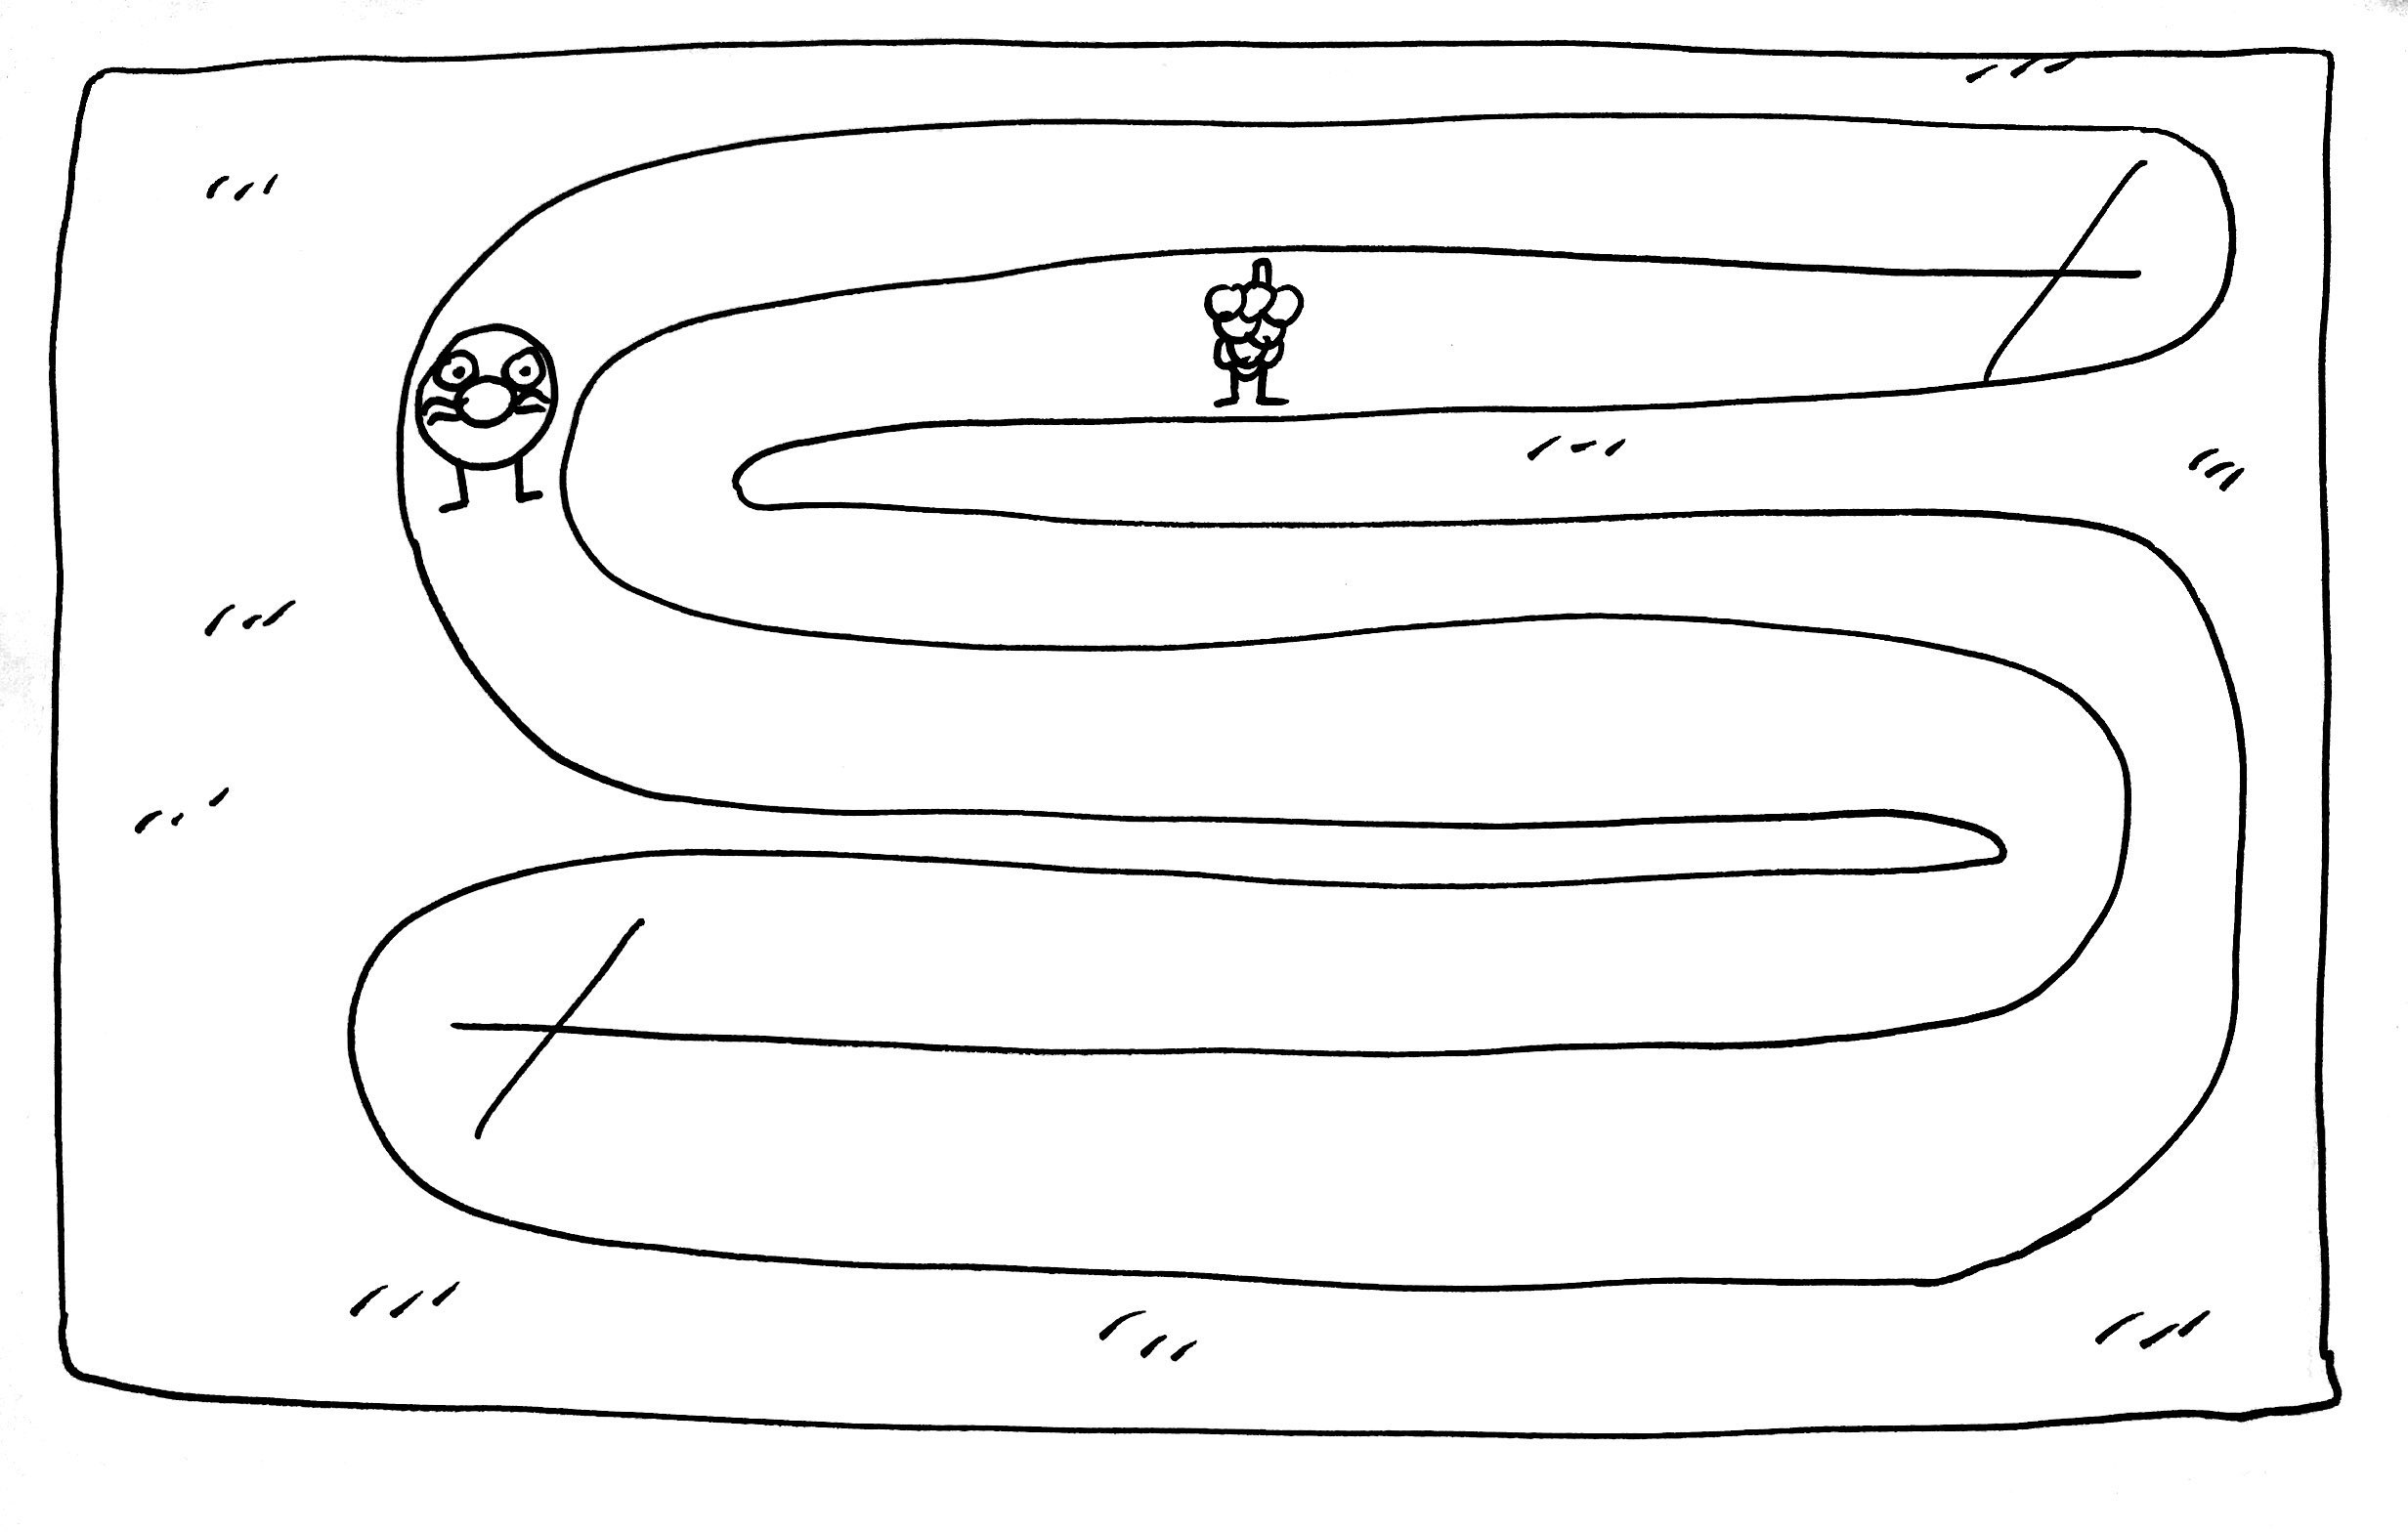
\includegraphics[scale=0.1]{Gambar/web5_gameplay2}
	\caption{Halaman pada \textit{PC} yang menampilkan lintasan lari dan karakter untuk dimainkan.}
	\label{fig:web5_gameplay2}
\end{figure}
	Untuk menampilkan karakter yang telah dipilih kelayar \textit{PC}, ada beberapa langkah yang harus dilakukan. Langkah-langkah tersebut akan dijelaskan sebagai berikut:
	\begin{itemize}
		\item \textit{Client} akan mengirimkan nilai dari karakter tertentu yang dipilih. Nilai tersebut dikirimkan melalui \textit{event} Socket.io yang dipancarkan dengan nama \textit{sendingChar}. \textit{Server} akan menangkap \textit{event} tersebut, kemudian akan memancarkan \textit{event} dengan nama \textit{startTheGame}, dimana \textit{event} tersebut akan ditangkap oleh \textit{host} untuk memulai permainan.
		
		\item \textit{Host} akan mulai menggambar karakter pada layar \textit{PC} setelah mendapatkan data-data yang dikirimkan melalui \textit{event startTheGame}.
		
		 
	\end{itemize}
	
	Untuk menampilkan karakter kelayar \textit{PC} saat proses animasi, dibutuhkan teknologi \textit{CanvasAPI} untuk menggambar karakter agar ditampilkan kelayar \textit{PC}. \textit{CanvasAPI} akan menciptakan objek \textit{canvas}, yang akan digunakan sebagai wadah dalam menggambar seluruh elemen yang diperlukan untuk permainan. Pada aplikasi permainan ini, objek \textit{Canvas} akan dibuat dengan ukuran panjang 900 piksel, dan lebar 600 piksel. Untuk memulai proses animasi, ada beberapa langkah yang harus dilakukan. Langkah-langkah tersebut dijelaskan sebagai berikut:
	\begin{enumerate}
		\item Objek \textit{Canvas} akan menetapkan properti \textit{globalCompositeOperation} dengan nilai \textit{destination-over}. Nilai tersebut akan menyebabkan objek yang ditaruh didalam \textit{canvas} saat ini, akan berada dibelakang objek yang sudah ditaruh sebelumnya.
		
		\item \textit{State}, yang merupakan keadaan dari objek \textit{canvas}, akan diubah ulang dengan cara menghilangkan seluruh objek yang berada didalam \textit{canvas}. Proses tersebut akan dilakukan dengan menggunakan \textit{method clearRect(0, 0, 900, 600)}. Dengan \textit{method} tersebut, seluruh elemen yang ada didalam \textit{canvas} dengan ukuran panjang 900 piksel dan lebar 600 piksel akan dihilangkan.  
		
		\item Proses pembaruan animasi akan dilakukan kepada seluruh pemain. Apabila pemain berada pada posisi x dan y tertentu, maka \textit{state} dari \textit{canvas} akan disimpan dengan menggunakan \textit{save()}. Setelah itu, karakter milik kedua pemain akan digambar ke \textit{canvas} dengan menggunakan \textit{drawImage()}. Setelah proses tersebut selesai, maka seluruh \textit{state} dari \textit{canvas} akan dikembalikan ke \textit{state} sebelumnya dengan menggunakan \textit{restore()}.
		
		\item Setelah proses pengecekan selesai, \textit{state} dari \textit{canvas} akan dikembalikan ke \textit{state} sebelumnya dengan menggunakan \textit{restore()}. Setelah itu akan dilakukan proses penggambaran lintasan lari dengan menggunakan drawImage(). Posisi lintasan lari yang digambar akan berada dibelakang gambar karakter yang sudah digambar sebelumnya. 
		
		\item Proses ini akan diulang kembali dari awal selama waktu permainan berjalan.
	\end{enumerate}

	\textbf{Smartphone}
	
	Halaman ini berfungsi sebagai pengendali untuk para pemain. Komponen halaman ini terdiri dari dua buah gambar telapak kaki yang berfungsi sebagai tombol. Pemain dapat menekan tombol berulang kali untuk menggerakan karakter yang ada pada halaman memulai permainan di \textit{PC}. Rancangan antarmuka halaman memulai permainan pada \textit{smartphone} dapat dilihat pada Gambar \ref{fig:mob5_play}.
	
\begin{figure}[H]
	\centering
	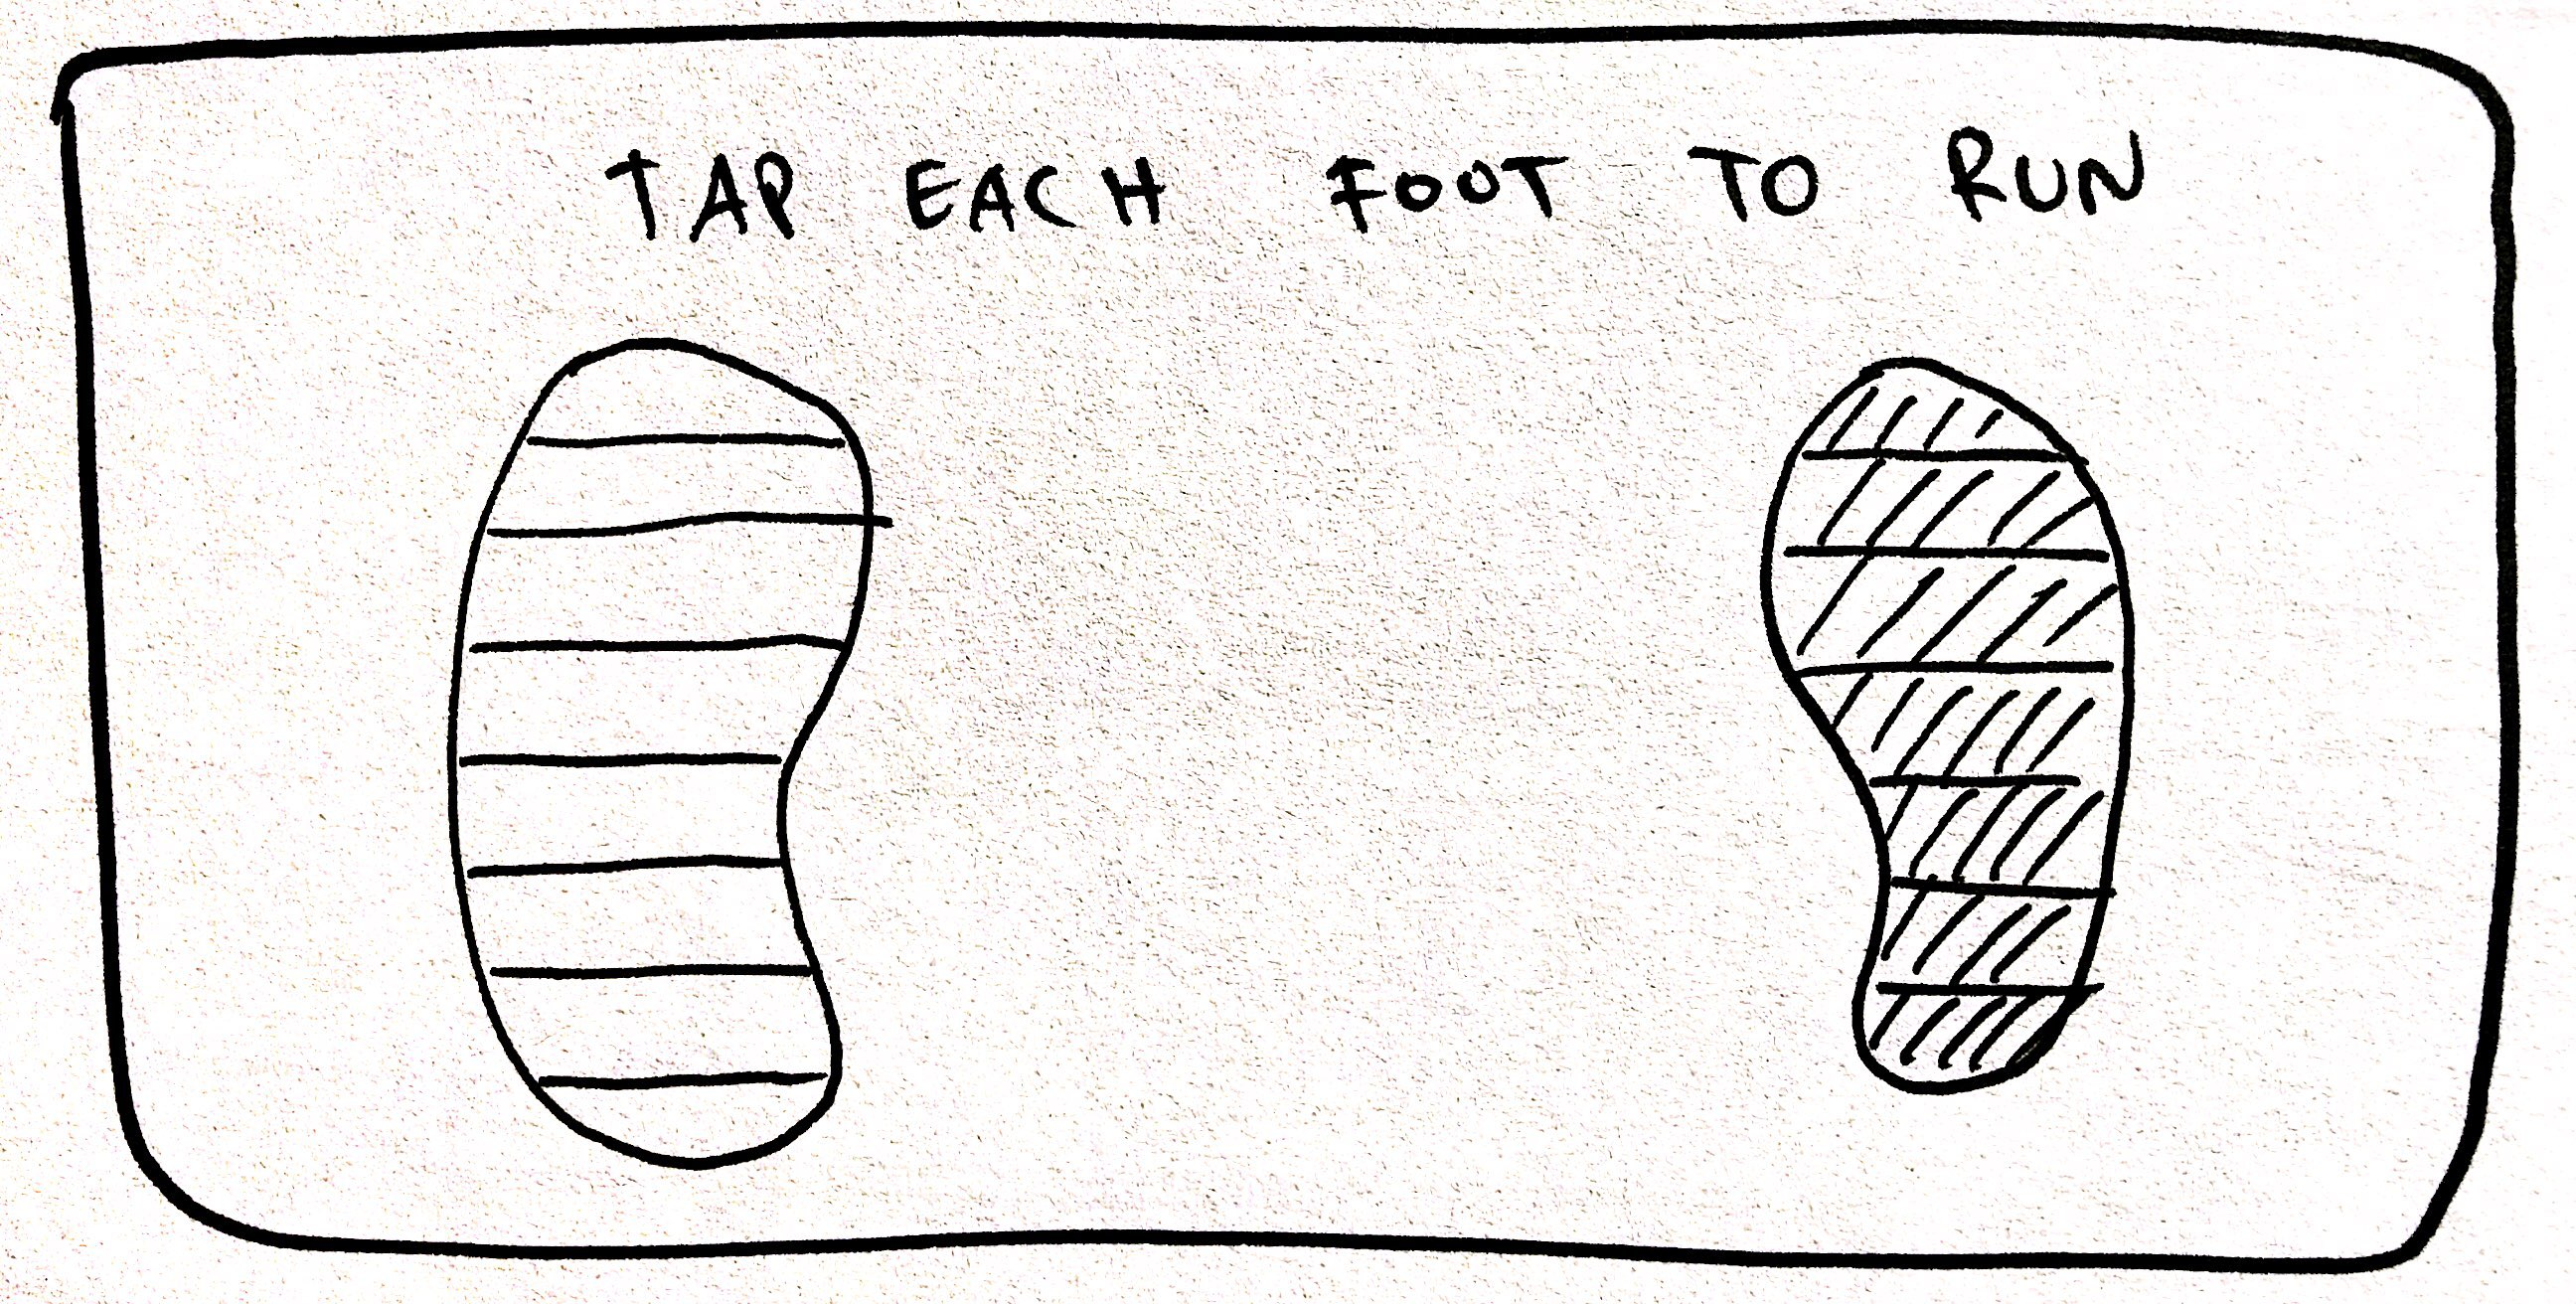
\includegraphics[scale=0.1]{Gambar/mob5_play}
	\caption{Halaman pada \textit{smartphone} yang menampilkan telapak kaki yang berfungsi sebagai pengendali.}
	\label{fig:mob5_play}
\end{figure}

\item Antarmuka halaman Mengakhiri Permainan

	\textbf{PC}
	
	Halaman ini menampilkan para pemenang yang telah berhasil menyelesaikan permainan. Setelah pemain selesai bermain, pemain dapat menekan tombol \textit{exit} untuk kembali ke halaman utama dan mengakhiri permainan. Rancangan antarmuka halaman mengakhiri permainan pada \textit{PC} dapat dilihat pada Gambar \ref{fig:web6_winning}.
	
\begin{figure}[H]
	\centering
	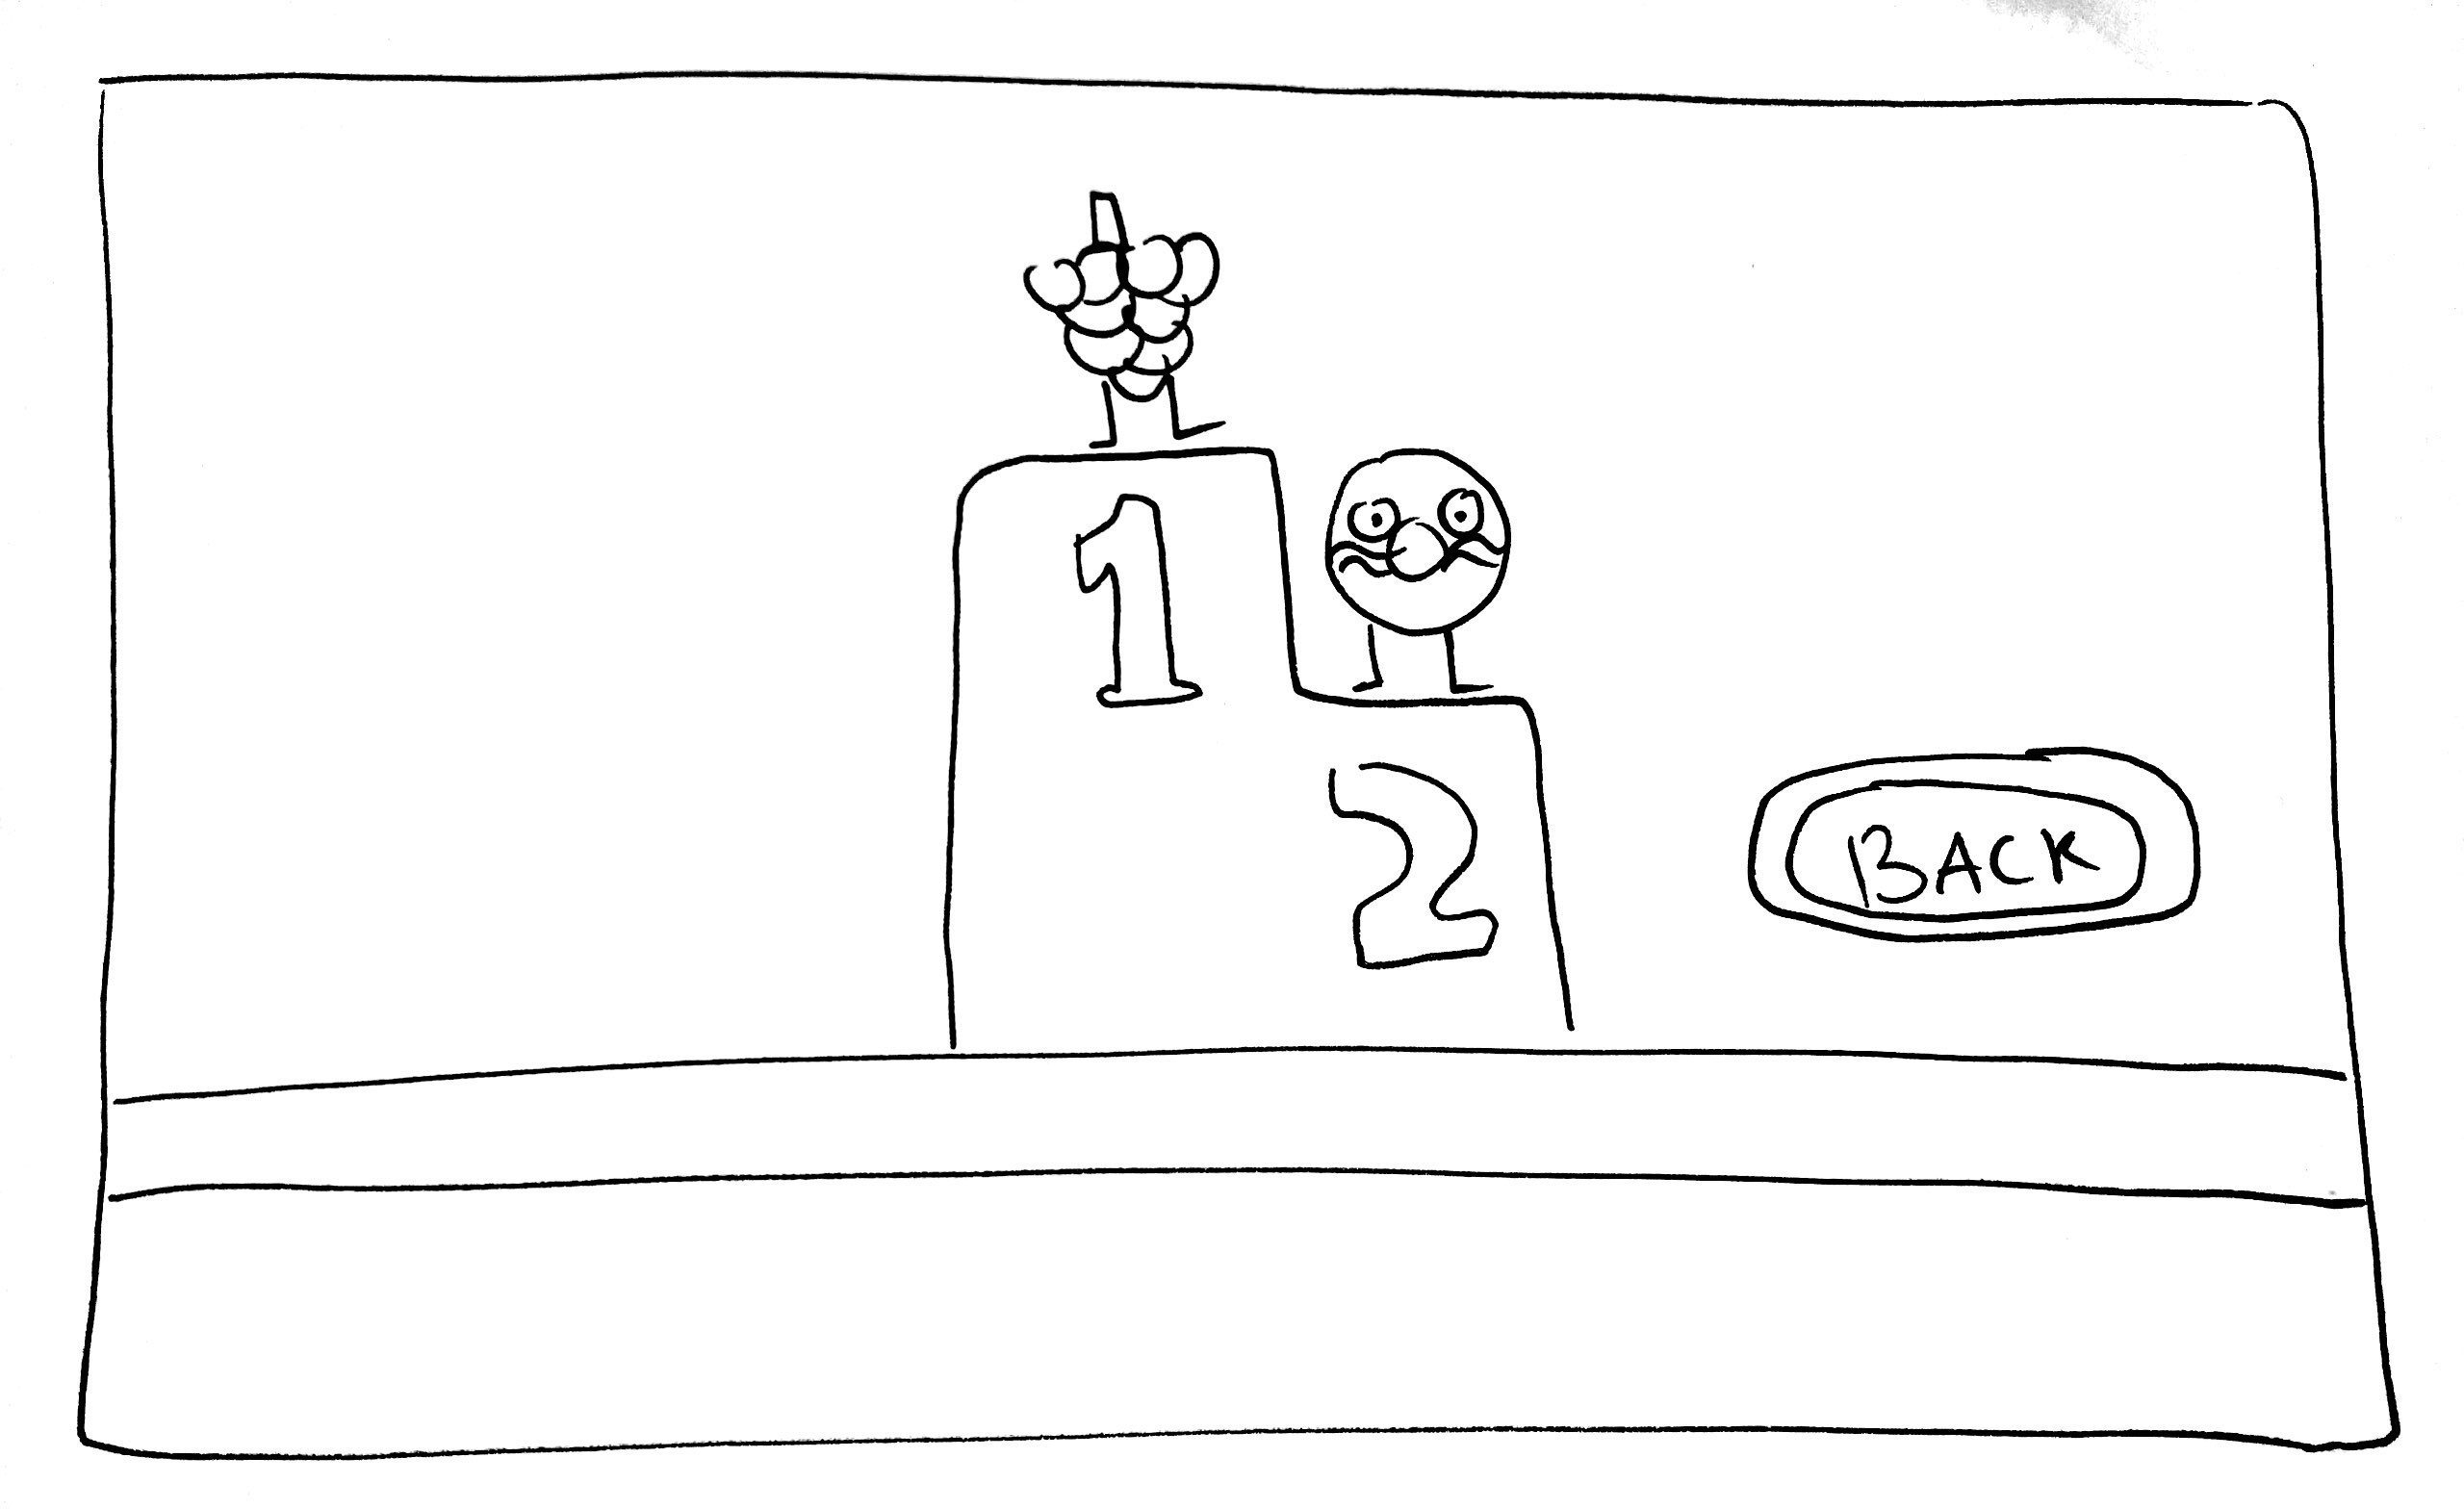
\includegraphics[scale=0.1]{Gambar/web6_winning}
	\caption{Halaman pada \textit{PC} yang menampilkan pemenang permainan.}
	\label{fig:web6_winning}
\end{figure}

	\textbf{Smartphone}
	
	Halaman ini menampilkan teks yang menandakan bahwa permainan telah selesai. Rancangan antarmuka halaman mengakhiri permainan pada \textit{smartphone} dapat dilihat pada Gambar \ref{fig:mob6_win}.
	
\begin{figure}[H]
	\centering
	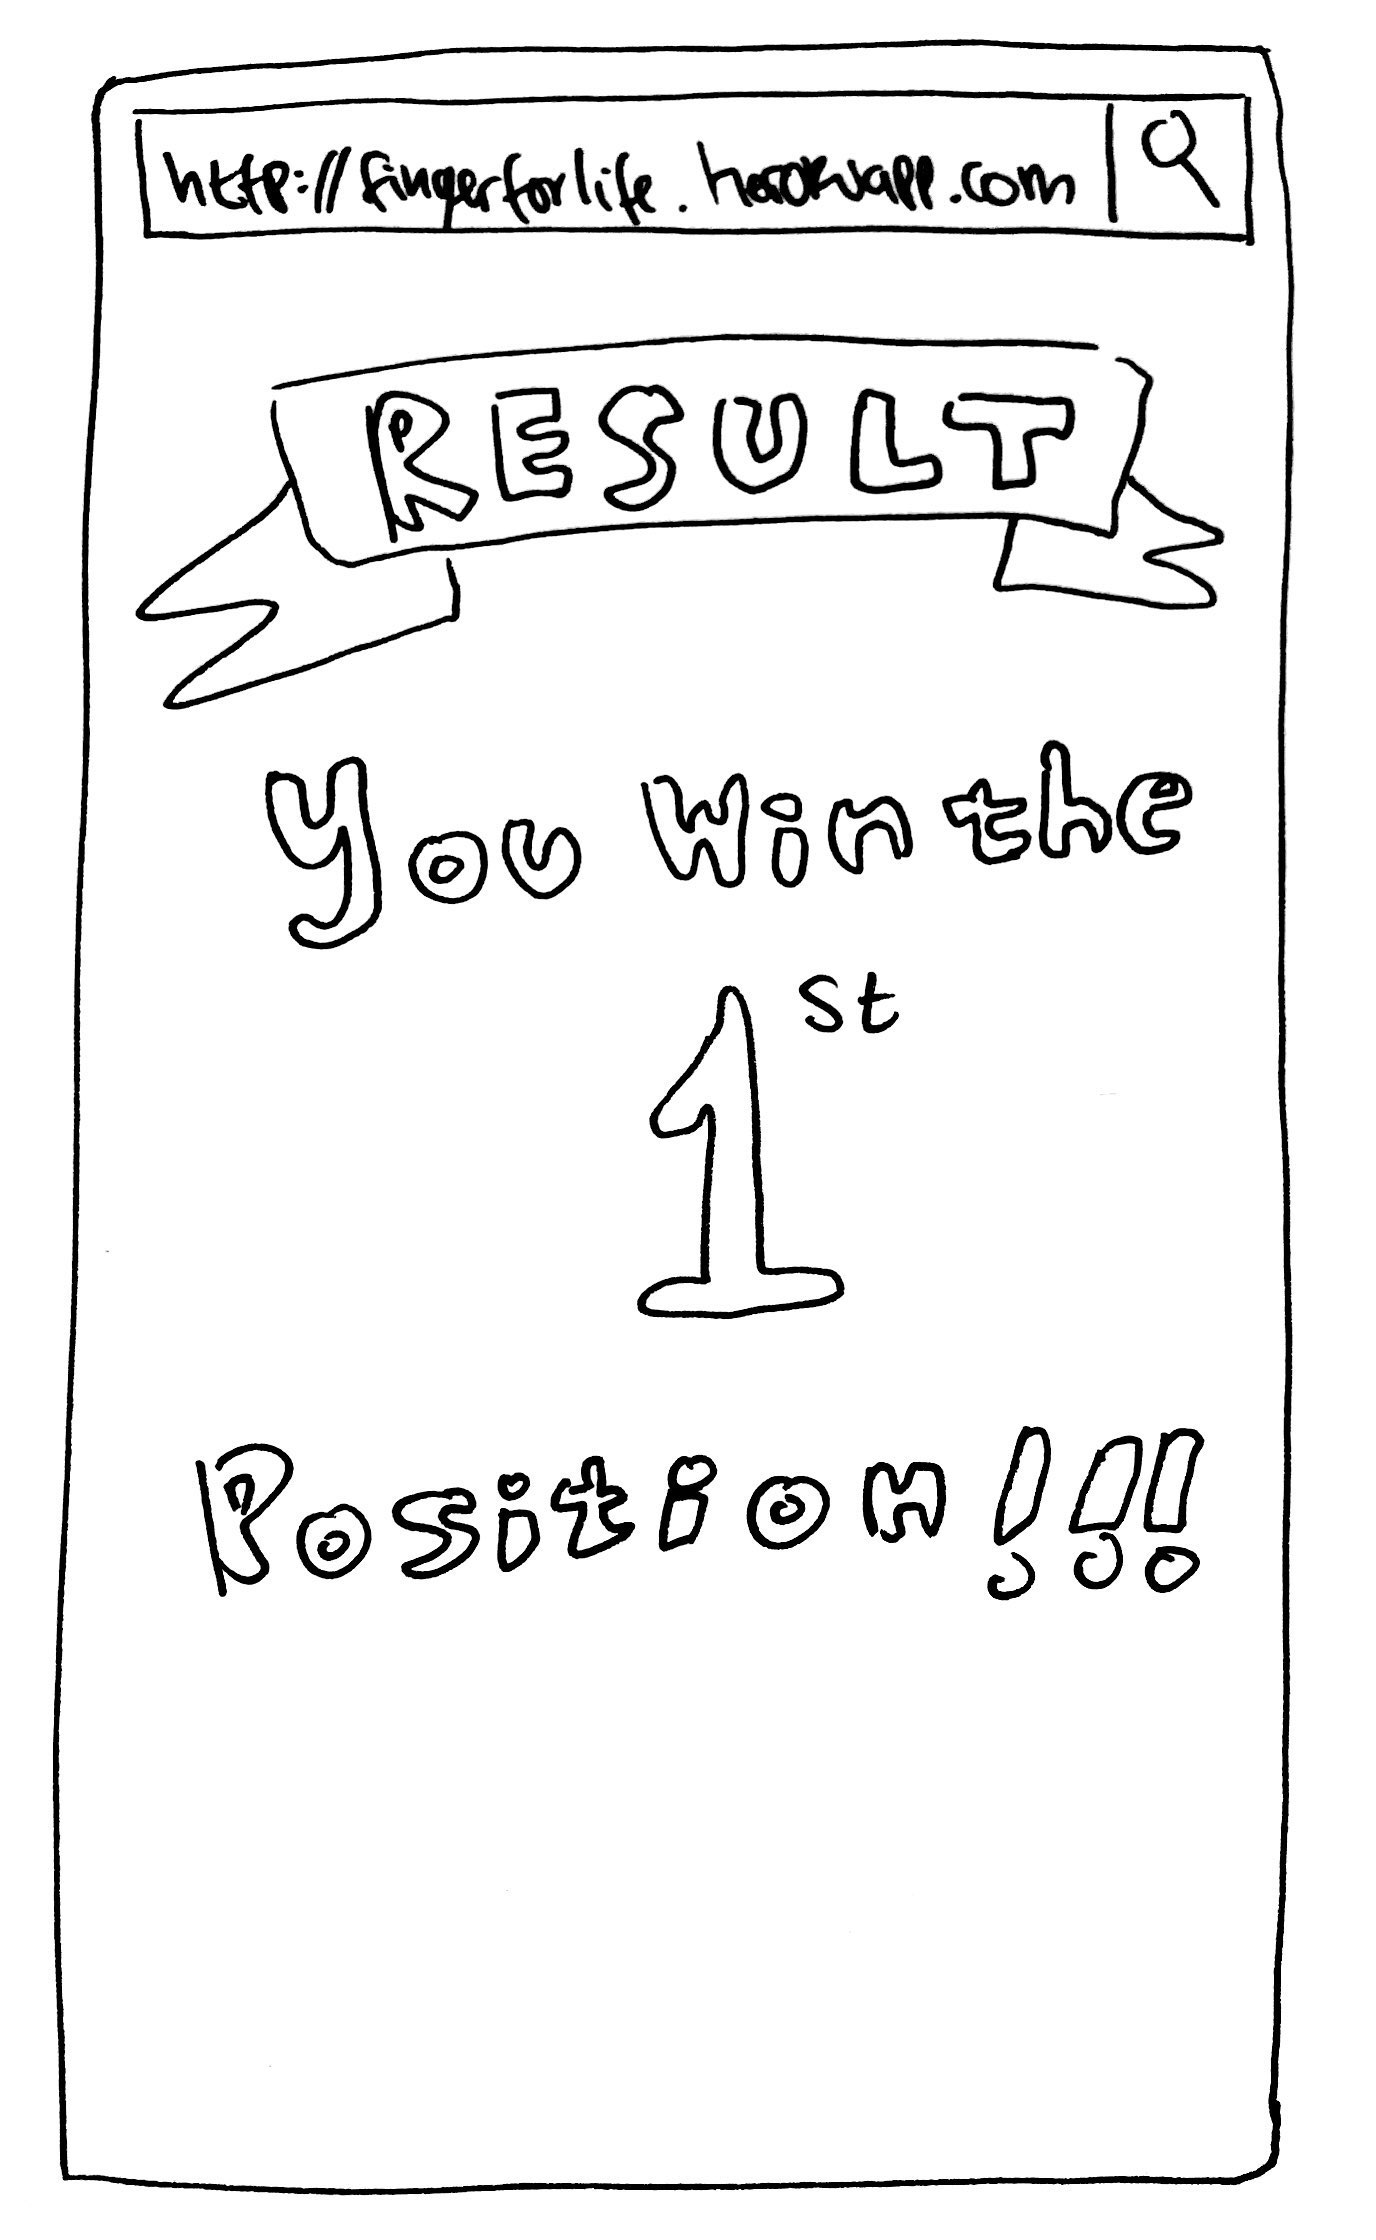
\includegraphics[scale=0.1]{Gambar/mob6_win}
	\caption{Halaman pada \textit{smartphone} yang menampilkan teks bahwa permainan telah selesai.}
	\label{fig:mob6_win}
\end{figure}
	
\end{enumerate}

\section{Perancangan Struktur Direktori}

Bagian ini akan membahas mengenai perancangan struktur direktori untuk membangun web. Struktur direktori meliputi beberapa direktori dan berkas yang memiliki fungsi berbeda-beda. Folder beserta berkas yang digunakan akan dijelaskan sebagai berikut:

\begin{figure}[H]
	\centering
	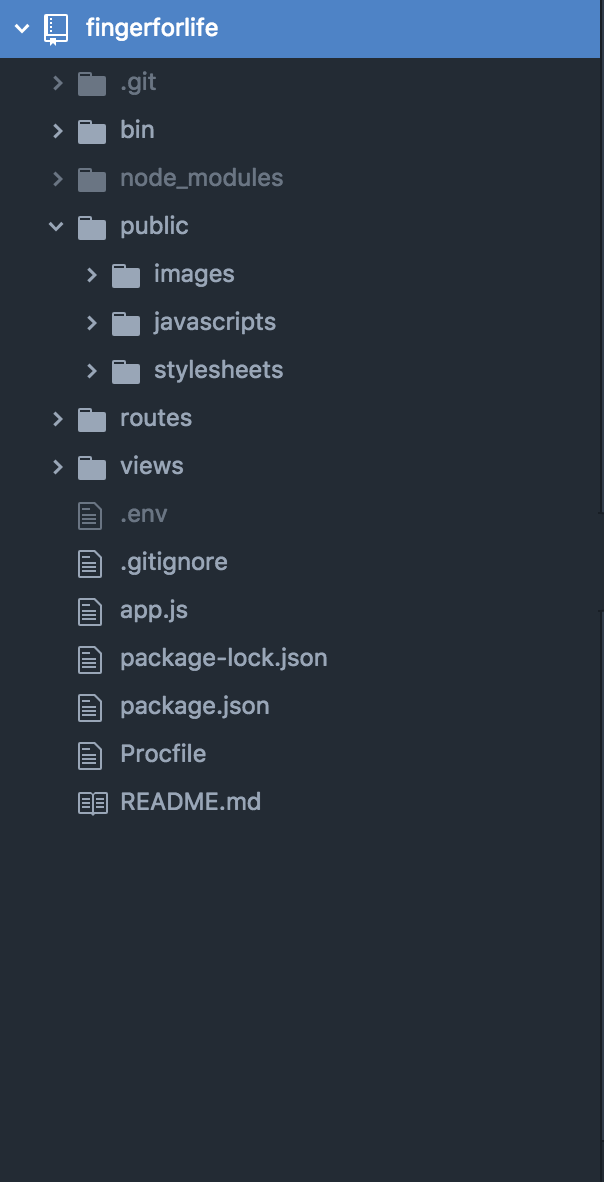
\includegraphics[scale=0.4]{Gambar/direktori}
	\caption{Direktori seluruh folder dan \textit{file}.}
	\label{fig:direktori}
\end{figure}

\begin{enumerate}
	\item \textbf{Direktori bin} \\
	
	\begin{figure}[H]
		\centering
		
\includegraphics[scale=0.4]{Gambar/direktori_bin}
		\caption{Isi direktori bin.}
		\label{fig:direktori_bin}
	\end{figure}
	
	Direktori ini berisi bagian-bagian yang berperan sebagai \textit{server}. Pada direktori ini terdapat direktori lain dan berkas yang berfungsi untuk menangani jalannya koneksi pada saat web diakses. Berikut merupakan isi dari direktori ini:
	\begin{enumerate}
		\item Direktori \textbf{utils} \\
		Direktori ini menyimpan berkas yang membantu proses berjalannya koneksi untuk \textit{server}. Isi dari direktori ini adalah sebagai berikut:
		\begin{itemize}
			\item Berkas \textbf{users.js}  \\
			Berkas ini merupakan suatu kelas yang berfungsi untuk menyimpan seluruh \textit{client} yang terkoneksi pada Socket.io. Seluruh data pengguna yang akan memainkan permainan web akan disimpan dan diatur oleh berkas ini.
			
			Kelas \textit{Users} memiliki konstruktor yang menginisialisasi variabel \textit{array} dengan nama \textit{userArray}. Variabel ini bertanggung jawab untuk menyimpan seluruh \textit{client} yang terkoneksi ke Socket.io.
			
			\textit{Method-method} yang dimiliki oleh berkas ini akan dijelaskan sebagai berikut:
			\begin{itemize}
				\item \textbf{addUser(id, room)} \\
				\textit{Method} ini akan menambahkan pengguna kedalam \textit{array} yang bernama \textit{userArray}. \\
				\textbf{Parameter:}
				\begin{itemize}
					\item \textbf{id}, identifikasi unik Socket.io milik pengguna.
					\item \textbf{room}, kode \textit{room} milik pengguna.
				\end{itemize}
				\textbf{Kembalian:} Objek \textit{Users}
				
				\item \textbf{IsRoomExist(room)} \\
				\textit{Method} ini akan memeriksa apakah parameter \textit{room} cocok dengan \textit{room} yang ada didalam \textit{userArray}. \\
				\textbf{Parameter:}
				\begin{itemize}
					\item \textbf{room}, kode \textit{room} yang akan dicek.
				\end{itemize}
				\item \textbf{Kembalian:} \textit{Integer}
				
				\item \textbf{getUser(id)} \\
				\textit{Method} ini akan mendapatkan pengguna dengan parameter \textit{id} yang cocok dengan \textit{id} yang ada didalam \textit{userArray}. \\
				\textbf{Parameter:}
				\begin{itemize}
					\item \textbf{id}, identifikasi unik Socket.io milik pengguna.
				\end{itemize}
				\textbf{Kembalian:} Objek Users
				
				\item \textbf{removeUser(id)} \\ 
				\textit{Method} ini akan menghapus pengguna dengan \textit{id} tertentu yang ada didalam \textit{userArray}. \\
				\textbf{Parameter:}
				\begin{itemize}
					\item \textbf{id}, identifikasi unik Socket.io milik pengguna.
				\end{itemize}
				\textbf{Kembalian:} Objek Users
				
				\item \textbf{getUserList(room)} \\
				\textit{Method} ini akan mengembalikan seluruh pengguna yang berada didalam \textit{room} yang cocok dengan parameter \textit{room}. \\
				\textbf{Parameter:}
				\begin{itemize}
					\item \textbf{room}, kode \textit{room} milik pengguna.
				\end{itemize}
				\textbf{Kembalian:} \textit{Array} objek Users
			\end{itemize}
			
		\end{itemize}
	
		\item \textbf{Berkas www} \\
		Berkas ini berfungsi sebagai \textit{server}. Seluruh koneksi yang tersambung dan terputus akan diatur oleh berkas ini. Komunikasi antara \textit{client} pun akan diatur oleh \textit{server}.
		
		Properti yang dimiliki oleh berkas ini akan dijelaskan sebagai berikut:
		\begin{itemize}
			\item \textbf{app}, variabel yang mendapatkan seluruh fitur dari berkas lain dengan nama \textit{app.js}.
			\item \textbf{http}, variabel yang mendapatkan seluruh fitur dari modul HTTP.
			\item \textbf{socketIO}, variabel yang mendapatkan seluruh fitur dari modul Socket.io.
			\item \textbf{{Users}}, variabel yang mendapatkan seluruh fitur dari kelas \textit{Users} dari berkas \textit{Users.js}.
			\item \textbf{port}, nilai \textit{port} yang akan dituju oleh \textit{server}.
			\item \textbf{server}, objek HTTP \textit{server} yang memiliki argumen variabel \textit{app} yang berfungsi sebagai \textit{handler} apabila ada koneksi yang masuk.
			\item \textbf{io}, objek Socket.io yang memiliki argumen \textit{server}. Objek ini akan menangkap \textit{event} dengan nama \textit{connection} yang dipancarkan oleh \textit{client}.
		\end{itemize}
	
		\textit{Method-method} yang dimiliki oleh berkas ini akan dijelaskan sebagai berikut:
		\begin{itemize}
			\item \textbf{normalizePort(val)} \\
			\textit{Method} ini berfungsi untuk mengubah bentuk parameter \textit{val} menjadi \textit{String, Integer}, atau \textit{false}. //
			\textbf{Parameter:}
			\begin{itemize}
				\item \textbf{val}, parameter \textit{port}
			\end{itemize}
			\textbf{Kembalian:} Objek \textit{String, Integer,} atau \textit{Boolean}. 
			
		\end{itemize}
	
		\textit{Event} Socket.io yang dimiliki berkas ini akan dijelaskan sebagai berikut:
		\begin{itemize}
			\item \textbf{io.on('connection', (socket) => {...})} \\
			Berfungsi untuk menangani suatu koneksi Socket.io yang baru tersambung.
			
			\item \textbf{socket.on('hostJoinRoom', (msg) => {...})} \\ 
			Berfungsi untuk menangkap \textit{event} \textbf{hostJoinRoom} yang dipancarkan oleh \textit{host} pada saat akan masuk kedalam room.
			
			\item \textbf{socket.on('sendingTheWinner', (winner) => {...})} \\
			Berfungsi untuk menangkap \textit{event} \textbf{sendingTheWinner} yang dipancarkan oleh \textit{client} setelah ada pemenang permainan.
			
			\item \textbf{socket.on('goBackHome', (msg) => {...})} \\
			Berfungsi untuk menangkap \textit{event} \textbf{goBackHome} yang dipancarkan oleh \textit{client} pada saat pemain menekan tombol \textit{exit} untuk kembali kehalaman utama.
			
			\item \textbf{socket.on('roomFull', (msg) => {...})} \\
			Berfungsi untuk menangkap \textit{event} \textbf{roomFull} yang dipancarkan oleh \textit{client} pada saat \textit{room} telah terisi penuh.
			
			\item \textbf{socket.on('selectingChar', (msg) => {...})} \\
			Berfungsi untuk menangkap \textit{event} \textbf{selectingChar} yang dipancarkan oleh \textit{client} pada saat karakter telah dipilih oleh pemain untuk menampilkan karakter kelayar \textit{PC}.
			
			\item \textbf{socket.on('sendingChar', (msg) => {...})} \\
			Berfungsi untuk menangkap \textit{event} \textbf{sendingChar} yang dipancarkan oleh \textit{client} pada saat karakter telah ditetapkan oleh pemain.
			
			\item \textbf{socket.on('charIsReady', (msg) => {...})} \\
			Berfungsi untuk menangkap \textit{event} \textbf{charIsReady} yang dipancarkan oleh \textit{client} pada saat kedua karakter telah ditetapkan oleh kedua pemain.
			
			\item \textbf{socket.on('stepClicked', (message) => {...})} \\
			Berfungsi untuk menangkap \textit{event} \textbf{stepClicked} yang dipancarkan oleh \textit{client} pada saat tombol telapak kaki ditekan oleh pemain.
			
			\item \textbf{socket.on('requestToJoin', (msg) => {...})} \\
			Berfungsi untuk menangkap \textit{event} \textbf{requestToJoin} yang dipancarkan oleh \textit{client} pada saat melakukan proses permintaan bergabung.
			
			\item \textbf{socket.on('disconnect', () => {...})} \\
			Berfungsi untuk menangkap \textit{event} \textbf{disconnect} yang dipancarkan oleh \textit{client} pada saat koneksi telah terputus.
 		\end{itemize}
	\end{enumerate}
	
	\item \textbf{Direktori public} \\
	
	\begin{figure}[H]
		\centering
		
\includegraphics[scale=0.4]{Gambar/direktori_public}
		\caption{Isi dari folder public.}
		\label{fig:direktori_public}
	\end{figure}
	
	Direktori ini menyimpan seluruh berkas yang memiliki sifat \textit{static}. Berikut akan dijelaskan isi dari direktori ini:
	\begin{enumerate}
		\item \textbf{Dirketori images} \\
		Direktori ini berisi gambar-gambar yang dibutuhkan untuk ditampilkan dibeberapa halaman yang terdapat didalam web. Berikut merupakan daftar isi dari gambar-gambar yang ada didalam direktori ini: 
		\begin{itemize}
			\item \textbf{BrocoDude.png} gambar karakter brokoli dengan ukuran besar, yaitu 1746 × 2454 piksel.
			\item \textbf{brocoDudeTiny.png} gambar karakter brokoli dengan ukuran kecil, yaitu 65 × 92 piksel.
			\item \textbf{DabuDonut.png} gambar karakter donat dengan ukuran besar, yaitu 1746 × 2454 piksel.
			\item \textbf{dabuDonut.png} gambar karakter donat dengan ukuran kecil, yaitu 65 × 92 piksel.
			\item \textbf{finga.png} gambar jari yang ditampilkan dihalaman awal.
			\item \textbf{GrapeYoda.png} gambar karakter anggur dengan ukuran besar, yaitu 1746 × 2454 piksel.
			\item \textbf{grapeYodaTiny.png} gambar karakter anggur dengan ukuran kecil, yaitu 65 × 92 piksel.
			\item \textbf{stepUp.png} gambar telapak kaki kiri yang ditampilkan dihalaman pengendali.
			\item \textbf{stepUpRight.png} gambar telapak kaki kanan yang ditampilkan dihalaman pengendali.
			\item \textbf{grapeYodaTiny.png} gambar karakter anggur dengan ukuran kecil.
			\item \textbf{SummerEgg.png} gambar karakter telur mata sapi dengan ukuran besar, yaitu 1746 × 2454 piksel.
			\item \textbf{summerEggTiny.png} gambar karakter telur mata sapi dengan ukuran kecil, yaitu 65 × 92 piksel.
			\item \textbf{timer1.png} gambar angka 1 yang ditampilkan saat hitungan mundur.
			\item \textbf{timer2.png} gambar angka 2 yang ditampilkan saat hitungan mundur.
			\item \textbf{timer3.png} gambar angka 3 yang ditampilkan saat hitungan mundur.
			\item \textbf{track.png} gambar lintasan saat permainan dimulai.
			\item \textbf{winning.png} gambar panggung saat sudah ada pemenang dalam permainan.
		\end{itemize}
	
		\item \textbf{Direktori javascripts} \\
		Direktori ini berisi bagian-bagian yang berfungsi untuk mengatur bagaimana perilaku web pada saat diakses oleh pengguna. Terdapat berbagai berkas dengan ekstensi \textbf{.js} yang memiliki fungsi berbeda-beda. Berikut akan dijelaskan isi dari folder ini:
		
		\begin{enumerate}
			\item \textbf{Direktori libs} \\
			Direktori ini berisi berkas yang berfungsi untuk mengatur pengiriman data melewati \textit{form}. Berikut isi dari folder ini:
			\begin{itemize}
				\item \textbf{jquery-3.3.1.min.js} \\ Berkas ini merupakan jQuery yang menyediakan fungsi-fungsi dalam pengiriman dan penerimaan data yang dilakukan \textit{client} dan \textit{server}. 
			\end{itemize}
		
			\item \textbf{charDesktopScript.js}, Berkas ini berfungsi untuk mengatur bagaimana perilaku halaman pemilihan karakter pada \textit{PC} pada saat diakses oleh \textit{client}.
			
			Atribut yang dimiliki oleh berkas ini adalah sebagai berikut:
			\begin{itemize}
				\item \textbf{marker}, \textit{integer} yang menandakan ada berapa pemain yang sudah menetapkan karakter.
				\item \textbf{playerData}, \textit{array} yang menyimpan objek pengguna dengan nilai karakter yang dipilihnya.
				\item \textbf{imageArray}, \textit{array} yang menyimpan daftar karakter yang dapat dipilih.
			\end{itemize}
		
			\textit{Method} yang dimiliki oleh berkas ini adalah sebagai berikut:
			\begin{itemize}
				\item \textbf{toGamePlayDesktop()} \\
				Berfungsi untuk memindahkan halaman kehalaman memulai permainan.
			\end{itemize}
		
			\textit{Event} Socket.io yang dimiliki oleh berkas ini adalah sebagai berikut:
			\begin{itemize}
				\item \textbf{socket.on('charSelecting', function(msg)\{\})} \\
				Berfungsi untuk menangkap \textit{event} charSelecting yang dipancarkan oleh \textit{server} pada saat karakter yang dipilih akan ditampilkan ke layar \textit{PC}.
				
				\item \textbf{socket.on('charSent', function(msg)\{\})} \\
				Berfungsi untuk menangkap \textit{event} charSent yang dipancarkan oleh \textit{server} untuk memeriksa apakah kedua pemain telah menetapkan karakter untuk pindah kehalaman selanjutnya.
			\end{itemize}
			
			\item \textbf{charMobileScript.js}, Berkas ini berfungsi untuk mengatur bagaimana perilaku halaman pemilihan karakter pada \textit{smarthone} pada saat diakses oleh \textit{client}.
			
			Atribut yang dimiliki oleh berkas ini adalah sebagai berikut:
			\begin{itemize}
				\item \textbf{mark}, \textit{integer} yang menandakan ada berapa pemain yang sudah menetapkan karakter.
			\end{itemize}
		
			\textit{Method} yang dimiliki oleh berkas ini adalah sebagai berikut:
			\begin{itemize}
				\item \textbf{selectChar()} \\
				Berfungsi untuk mengirimkan nilai karakter yang telah dipilih oleh pemain.
			\end{itemize}
			
			\textit{Event} yang dimiliki oleh berkas ini adalah sebagai berikut:
			\begin{itemize}
				\item \textbf{socket.on('charSent', function(msg){})} \\ 
				Berfungsi untuk menangkap \textit{event} charSent yang dipancarkan oleh \textit{server} untuk memeriksa apakah kedua pemain telah menetapkan karakter untuk pindah kehalaman selanjutnya.
				
				\item \textbf{socket.emit('selectingChar', {val, id})} \\
				Berfungsi untuk memancarkan \textit{event} selectingChar saat pemain telah memilih karakter. Data yang dikirimkan adalah:
				\begin{itemize}
					\item \textbf{val}, nilai karakter berupa \textit{integer}.
					\item \textbf{id}, identifikasi unik Socket.io milik pemain.
				\end{itemize}
			
				\item \textbf{socket.on('sendingChar', {val, id, marker})} \\
				Berfungsi untuk memancarkan \textit{event} sendingChar saat pemain telah menetapkan karakter yang dipilih. Data yang dikirimkan adalah:
				\begin{itemize}
					\item \textbf{val}, nilai karakter berupa \textit{integer}.
					\item \textbf{id}, identifikasi unik Socket.io milik pemain.
					\item \textbf{marker}, \textit{integer} penanda seorang pemain telah menetapkan karakter.
				\end{itemize}
			\end{itemize}
			
			\item \textbf{gamePlayDesktopScript.js}, Berkas ini berfungsi untuk mengatur bagaimana perilaku halaman permainan di \textit{PC browser} pada saat diakses oleh \textit{client}.
			
			Atribut yang dimiliki oleh berkas ini adalah sebagai berikut:
			\begin{itemize}
				\item \textbf{canvas}, elemen \textit{canvas} yang ada pada berkas HTML.
				\item \textbf{ctx} , menyimpan fungsi-fungsi konteks 2d milik \textit{Canvas API} untuk pemain pertama.
				\item \textbf{ctx2}, menyimpan fungsi-fungsi konteks 2d milik \textit{Canvas API} untuk pemain kedua.
				\item \textbf{track}, gambar lintasan lari.
				\item \textbf{timer1}, gambar angka 1 yang akan digunakan pada \textit{countdown}.
				\item \textbf{timer2}, gambar angka 2 yang akan digunakan pada \textit{countdown}.
				\item \textbf{timer3}, gambar angka 3 yang akan digunakan pada \textit{countdown}.
				\item \textbf{player1Char},  gambar karakter milik pemain pertama.
				\item \textbf{player2Char}, gambar karakter milik pemain kedua.
				\item \textbf{dataOfPlayer}, menyimpan data kedua pemain.
				\item \textbf{player1Val}, menyimpan nilai karakter pemain pertama yang telah dipilih.
				\item \textbf{player2Val}, menyimpan nilai karakter pemain kedua yang telah dipilih.
				\item \textbf{winner}, menyimpan pemain pemenang.
				\item \textbf{timerArray}, menyimpan kumpulan gambar angka untuk proses \textit{coundown}.
				\item \textbf{charArray}, menyimpan kumpulan gambar karakter.
				\item \textbf{arrOfPlayerChar}, menyimpan kedua karakter yang telah dipilih oleh pemain.
				\item \textbf{aniFrame}, menyimpan \textit{animation frame} yang digunakan untuk proses animasi karakter pemain pertama.
				\item \textbf{aniFrame2}, menyimpan \textit{animation frame} yang digunakan untuk proses animasi karakter pemain kedua.
				\item \textbf{progressPlayer1}, menyimpan kemajuan suatu posisi karakter yang digerakan pada lintasan lari milik pemain pertama.
				\item \textbf{progressPlayer2}, menyimpan kemajuan suatu posisi karakter yang digerakan pada lintasan lari milik pemain kedua.
				\item \textbf{xPosition1}, menyimpan posisi karakter pemain pertama pada sumbu x.
				\item \textbf{yPosition1}, menyimpan posisi karakter pemain pertama pada sumbu y.
				\item \textbf{xPosition2}, menyimpan posisi karakter pemain kedua pada sumbu x.
				\item \textbf{yPosition2}, menyimpan posisi karakter pemain kedua pada sumbu y.
			\end{itemize}
			
			\textit{Method} yang dimiliki oleh berkas ini adalah sebagai berikut:
			\begin{itemize}
				\item \textbf{init()} \\
				Berfungsi untuk menggambar lintasan lari diawal permainan.
				
				\item \textbf{beginCountDown(beginCounter, msg)} \\
				Berfungsi untuk memulai hitungan mundur dengan menggambar angka tiga hingga satu kelayar permainan.
				
				\item \textbf{drawChar(data)} \\
				Berfungsi untuk menggambar karakter milik pemain diatas lintasan lari.
				
				\item \textbf{beginGamePlay()} \\
				Berfungsi untuk memulai permainan.
				
				\item \textbf{reachFinishLine(player)} \\
				Berfungsi untuk mencatat pemain mana yang sampai pada garis akhir duluan.
				
				\item \textbf{toWinningPage()} \\
				Berfungsi untuk memindahkan halaman ke halaman pemenang.
				
				\item \textbf{readyPlayerOne()} \\
				Berfungsi untuk menggerakan karakter pemain pertama pada saat tombol telapak kaki ditekan.
				
				\item \textbf{readyPlayerTwo()} \\
				Berfungsi untuk menggerakan karakter pemain kedua pada saat tombol telapak kaki ditekan.
			\end{itemize}
			
			\textit{Event} yang dimiliki oleh berkas ini adalah sebagai berikut:
			\begin{itemize}
				\item \textbf{socket.on('moveThePlayer', function(msg){...})}\\
				Berfungsi untuk menangkap \textit{event} moveThePlayer yang dipancarkan oleh \textit{server} saat tombol telapak kaki ditekan oleh pemain.
				
				\item \textbf{socket.on('startTheGame', function(msg){...})}\\
				Berfungsi untuk menangkap \textit{event} startTheGame yang dipancarkan oleh \textit{server} pada saat akan memulai permainan dengan menggambar aset-aset yang dibutuhkan ke layar \textit{PC}.
				
				\item \textbf{socket.on('toWinnerPage', function(){})} \\
				Berfungsi untuk menangkap \textit{event} toWinnerPage yang dipancarkan oleh \textit{server} yang memindahkan halaman ke halaman pemenang.
				
				\item \textbf{socket.emit('sendingTheWinner', {playerWin,playerCharArr})} \\
				Berfungsi untuk memancarkan \textit{event} sendingTheWinner pada saat pemain telah mencapai garis akhir. Data yang dikirimkan adalah:
				\begin{itemize}
					\item \textbf{playerWin}, pemenang yang mencapai garis akhir lebih dulu.
					\item \textbf{playerCharArr}, nilai dari kedua karakter milik para pemain.
				\end{itemize}
			\end{itemize}
			
			\item \textbf{gamePlayMobileScript.js}, Berkas ini berfungsi untuk mengatur bagaimana perilaku halaman permainan di \textit{mobile browser} pada saat diakses oleh \textit{client}.
			
			Atribut yang dimiliki oleh berkas ini adalah sebagai berikut:
			\begin{itemize}
				\item \textbf{stepLeftHtml}, Elemen HTML berupa gambar telapak kaki.
				\item \textbf{instructionEl}, Elemen HTML berupa teks instruksi.
			\end{itemize}
			
			\textit{Method} yang dimiliki oleh berkas ini adalah sebagai berikut:
			\begin{itemize}
				\item \textbf{stepClicked()} \\
				Berfungsi untuk menangani aksi menekan tombol telapak kaki oleh pemain.
				
				\item \textbf{moveToWinPage()} \\
				Berfungsi untuk memindahkan halaman ke halaman pemenang.
				
				\item \textbf{showInstruction(beginCounter)} \\
				Berfungsi untuk menampilkan instruksi kelayar permainan.\\
				\textbf{Parameter:}
				\begin{itemize}
					\item \textbf{beginCounter}, \textit{integer} yang menunjukan berapa detik instruksi akan ditampilkan.
				\end{itemize}
			\end{itemize}
			
			\textit{Event} yang dimiliki oleh berkas ini adalah sebagai berikut:
			\begin{itemize}
				\item \textbf{socket.on('startTheGame', function()\{...\})}\\
				Berfungsi untuk menangkap \textit{event} startTheGame yang dipancarkan oleh \textit{server} saat permainan akan segera dimulai.
				
				\item \textbf{socket.on('toWinnerPage', function()\{...\})}\\
				Berfungsi untuk menangkap \textit{event} toWinnerPage yang dipancarkan oleh \textit{server} pada saat permainan telah selesai.
				
				\item \textbf{socket.emit('stepClicked',\{playerId\})} \\
				Berfungsi untuk memancarkan \textit{event} stepClicked pada saat pemain menekan tombol telapak kaki dilayar \textit{smartphone}.
			\end{itemize}
			
			\item \textbf{homeScript.js}, Berkas ini berfungsi untuk mengatur bagaimana perilaku halaman utama di \textit{PC browser} dan \textit{mobile browser} pada saat diakses oleh \textit{client}.
			
			Atribut yang dimiliki oleh berkas ini adalah sebagai berikut:
			\begin{itemize}
				\item \textbf{bg}, elemen HTML berupa \textit{div} dengan nama kelas \textit{stage-area}.
				\item \textbf{titleHtml}, elemen HTML berupa \textit{div} dengan nama \textit{id homePage}.
			\end{itemize}
			
			\textit{Method} yang dimiliki oleh berkas ini adalah sebagai berikut:
			\begin{itemize}
				\item \textbf{startClicked()} \\
				Berfungsi untuk memindahkan halaman menuju halaman proses permintaan bergabung pada \textit{PC}.
				
				\item \textbf{joinClicked()} \\
				Berfungsi untuk memindahkan halaman menuju halaman proses permintaan bergabung pada \textit{smartphone}.
			\end{itemize}
			
			\item \textbf{mobileScript.js}, Berkas ini berfungsi untuk mengatur bagaimana perilaku halaman proses permintaan koneksi di \textit{mobile browser} pada saat diakses oleh \textit{client}.
			
			Atribut yang dimiliki oleh berkas ini adalah sebagai berikut:
			\begin{itemize}
				\item \textbf{socket}, variabel koneksi Socket.io
			\end{itemize}
			
			\textit{Method} yang dimiliki oleh berkas ini adalah sebagai berikut:
			\begin{itemize}
				\item \textbf{requestToJoin()} \\ 
				Berfungsi untuk melakukan proses permintaan bergabung saat pengguna menekan tombol \textit{send}.
				
				\item \textbf{toCharMobile()} \\
				Berfungsi untuk memindahkan halaman ke halaman pemilihan karakter.
			\end{itemize}
			
			\textit{Event} yang dimiliki oleh berkas ini adalah sebagai berikut:
			\begin{itemize}
				\item \textbf{socket.on('connect',function()/{.../})} \\
				Berfungsi untuk menangkap \textit{event} connect yang dipancarkan apabila \textit{client} berhasil tersambung ke Socket.io.
				
				\item \textbf{socket.on('joinSucceed', function(msg)\{...\})} \\
				Berfungsi untuk menangkap \textit{event} joinSucceed yang dipancarkan oleh \textit{server} apabila \textit{client} berhasil bergabung kedalam \textit{room}.
				
				\item \textbf{socket.on('joinRejected', function(msg)\{...\})} \\
				Berfungsi untuk menangkap \textit{event} joinRejected yang dipancarkan oleh \textit{server} apabila \textit{client} tidak berhasil bergabung kedalam \textit{room}.
				
				\item \textbf{socket.on('toCharPage')} \\
				Berfungsi untuk menangkap \textit{event} toCharPage yang dipancarkan oleh \textit{server} pada saat akan berpindah halaman ke halaman pemilihan karakter.
			\end{itemize}
			
			\item \textbf{syncScript.js}, Berkas ini berfungsi untuk mengatur bagaimana perilaku halaman proses permintaan koneksi di \textit{PC browser} pada saat diakses oleh \textit{client}.
			
			Atribut yang dimiliki oleh berkas ini adalah sebagai berikut:
			\begin{itemize}
				\item \textbf{socket}, variabel koneksi Socket.io.
				\item \textbf{player}, \textit{integer} yang menunjukan pemain urutan keberapa.
				\item \textbf{players}, \textit{array} yang menyimpan data para pemain.
				\item \textbf{text}, \textit{integer} kode \textit{room}. 
			\end{itemize}
			
			\textit{Method} yang dimiliki oleh berkas ini adalah sebagai berikut:
			\begin{itemize}
				\item \textbf{toCharDesk()} \\
				Berfungsi untuk memindahkan halaman ke halaman pemilihan karakter pada \textit{PC}.
				
				\item \textbf{getRandInt()} \\
				Berfungsi untuk membangkitkan kode \textit{room} berupa \textit{integer} secara acak.
				
				\item \textbf{requestAccepted(msg)} \\
				Berfungsi untuk memasukan data \textit{client} kedalam \textit{array} pada saat telah tersambung ke Socket.io.
			\end{itemize}
			
			\textit{Event} yang dimiliki oleh berkas ini adalah sebagai berikut:
			\begin{itemize}
				\item \textbf{socket.on('connect', function()\{\})} \\
				Berfungsi untuk menangkap \textit{event} connect pada saat \textit{client} telah berhasil tersambung ke Socket.io.
				
				\item \textbf{socket.on('requestAccepted',function(msg)\{\})} \\
				Berfungsi untuk menangkap \textit{event} requestAccepted yang dipancarkan oleh \textit{server} pada saat \textit{client} telah berhasil bergabung kedalam \textit{room}.
				
				\item \textbf{socket.on('toCharPage', function()\{\})} \\
				Berfungsi untuk menangkap \textit{event} toCharPage yang dipancarkan oleh \textit{server} pada saat akan memindahkan halaman ke halaman pemilihan karakter pada \textit{smartphone}
				
				\item \textbf{socket.emit('hostJoinRoom',\{id, room\})} \\
				Berfungsi untuk memancarkan \textit{event} hostJoinRoom saat \textit{host} telah bergabung kedalam \textit{room}. Data yang dikirimkan adalah:
				\begin{itemize}
					\item \textbf{id} identifikasi unik Socket.io milik \textit{client}
					\item \textbf{room} kode \textit{room} milik \textit{client}
				\end{itemize}
			
				\item \textbf{socket.emit('roomFull', \{room\})} \\
				Berfungsi untuk memancarkan \textit{event} hostJoinRoom pada saat \textit{room} sudah terisi penuh.	
				
			\end{itemize}
			
			\item \textbf{winningDesktopScript.js}, Berkas ini berfungsi untuk mengatur bagaimana perilaku halaman saat permainan telah selesai di \textit{PC browser} pada saat diakses oleh \textit{client}.
			
			Atribut yang dimiliki oleh berkas ini adalah sebagai berikut:
			\begin{itemize}
				\item \textbf{winCanvas}
				\item \textbf{winCtx}
				\item \textbf{podium}
				\item \textbf{winnerCharArr}
			\end{itemize}
			
			\textit{Method} yang dimiliki oleh berkas ini adalah sebagai berikut:
			\begin{itemize}
				\item \textbf{drawStage()} \\
				Berfungsi untuk menggambar podium ke layar permainan.
				
				\item \textbf{drawWinner(winner)} \\
				Berfungsi untuk menggambar para pemenang permainan.
				
				\item \textbf{drawFirstWinner(firstWinner)} \\
				Berfungsi untuk menggambar pemenang pertama.
				
				\item \textbf{drawSecondWinner(secondWinner)} \\
				Berfungsi untuk menggambar pemenang kedua.
				
				\item \textbf{toHomePage()} \\
				Berfungsi untuk memindahkan halaman ke halaman awal.
			\end{itemize}
			
			\textit{Event} yang dimiliki oleh berkas ini adalah sebagai berikut:
			\begin{itemize}
				\item \textbf{socket.on('getTheWinner',function(msg)\{\})} \\
				Berfungsi untuk menangkap \textit{event} getTheWinner yang dipancarkan oleh \textit{server} pada saat permainan selesai.
				
				\item \textbf{socket.on('backHome', function()\{\})}  \\
				Berfungsi untuk menangkap \textit{event} backHome yang dipancarkan oleh \textit{server} untuk memindahkan halaman ke halaman awal.
				
				\item \textbf{socket.emit('goBackHome', 'back home')} \\
				Berfungsi untuk memancarkan \textit{event} goBackHome pada saat pemain menekan tombol \textit{exit}. 
				 
			\end{itemize}
			
			\item \textbf{winningMobileScript.js}, Berkas ini berfungsi untuk mengatur bagaimana perilaku halaman saat permainan telah selesai di \textit{mobile browser} pada saat diakses oleh \textit{client}.
			
			Atribut yang dimiliki oleh berkas ini adalah sebagai berikut:
			\begin{itemize}
				\item \textbf{gameOverEl}, elemen HTML berupa teks.
			\end{itemize}
			
			\textit{Method} yang dimiliki oleh berkas ini adalah sebagai berikut:
			\begin{itemize}
				\item \textbf{showGameOver()} \\
				Berfungsi untuk menampilkan teks yang menandakan permainan sudah selesai.
				
				\item \textbf{backToHome()} \\
				Berfungsi untuk memindahkan halaman ke halaman awal.
			\end{itemize}
			
			\textit{Event} yang dimiliki oleh berkas ini adalah sebagai berikut:
			
		\end{enumerate}
		\item \textbf{Folder stylesheets} \\ 
		Folder ini berisi bagian-bagian yang berfungsi untuk menghias setiap halaman yang terdapat didalam web. Pada folder ini terdapat berbagai berkas dengan ekstensi \textbf{.css}. Berikut akan dijelaskan isi dari folder ini:
		
		\begin{enumerate}
			\item \textbf{charDesktopStyle.css}, Berkas ini berfungsi untuk menghias halaman pemilihan karakter pada \textit{PC browser}.
			
			\item \textbf{charMobileStyle.css}, Berkas ini berfungsi untuk menghias halaman pemilihan karakter pada \textit{mobile browser}.
			
			\item \textbf{gamePlayDesktopStyle.css}, Berkas ini berfungsi untuk menghias halaman permainan pada \textit{PC browser}.
			
			\item \textbf{gamePlayMobileStyle.css}, Berkas ini berfungsi untuk menghias halaman permainan pada \textit{mobile browser}.
			
			\item \textbf{homeStyle.css}, Berkas ini berfungsi untuk menghias halaman utama pada \textit{PC browser} dan \textit{mobile browser}.
			
			\item \textbf{mobileStyle.css}, Berkas ini berfungsi untuk menghias halaman proses permintaan koneksi pada \textit{mobile browser}.
			
			\item \textbf{Nickname\_DEMO.otf\footnote{\url{http://pizzadude.dk/site/fonts/nickname}, diakses 12 September 2018}}, Berkas ini berfungsi sebagai tipe \textit{font} yang digunakan di beberapa halaman yang terdapat pada web.
			
			\item \textbf{syncStyle.css}, Berkas ini berfungsi untuk menghias halaman proses permintaan koneksi pada \textit{PC browser}.
			
			\item \textbf{winningDesktopStyle.css}, Berkas ini berfungsi untuk menghias halaman saat permainan telah selesai pada \textit{mobile browser}.
			
			\item \textbf{winningMobileStyle.css}, Berkas ini berfungsi untuk menghias halaman saat permainan telah selesai pada \textit{mobile browser}.
			
			
		\end{enumerate}
	\end{enumerate}
	
	\item \textbf{Folder routes} \\
	
	\begin{figure}[H]
		\centering
		
\includegraphics[scale=0.4]{Gambar/direktori_routes}
		\caption{Isi dari folder routes}
		\label{fig:direktori_routes}
	\end{figure}
	
	Folder ini berisi bagian-bagian yang berperan sebagai \textit{middleware}. Berikut merupakan isi dari folder ini:
	\begin{itemize}
		\item \textbf{homeRoutes.js}, berkas ini berfungsi sebagai \textit{middleware} yang menampilkan halaman utama pada saat \textit{client} mengakses alamat web. Berkas ini akan digunakan oleh berkas \textbf{app.js} yang berperan sebagai modul utama.
	\end{itemize}

	\item \textbf{Folder views} \\
	
	\begin{figure}[H]
		\centering
		
\includegraphics[scale=0.4]{Gambar/direktori_views}
		\caption{Isi dari folder views}
		\label{fig:direktori_views}
	\end{figure}
	
	Folder ini berisi bagian-bagian yang berfungsi untuk menampilkan halaman-halaman kepada \textit{client}. Folder ini memiliki berkas dengan ekstensi \textbf{.ejs}. Sama seperti ekstensi \textbf{.html}, ekstensi tersebut akan menampilkan berbagai tampilan dengan menggunakan \textit{syntax} \textbf{.html}. Berikut merupakan isi dari folder ini:
	
	\begin{enumerate}
		\item \textbf{error.ejs}, berkas ini berisi \textit{template} yang akan menampilkan halaman \textit{error} apabila terjadi kesalahan dalam mengakses web. Halaman ini akan ditampilkan oleh \textit{router}.
		
		\item \textbf{home.ejs}, berkas ini berisi \textit{template} yang akan menampilkan halaman awal pada saat pengguna mengakses web. Halaman ini akan ditampilkan oleh \textit{router}.
	\end{enumerate}
	
	
	\item \textbf{Berkas app.js} \\ 
	Berkas ini berfungsi sebagai modul utama, yang mengatur akses dari berbagai folder dan berkas yang ada pada struktur web ini.
	
%	\item \textbf{Berkas .gitignore} \\
%	Berkas ini berfungsi untuk kebutuhan penyimpanan direktori di \textit{github}, dimana isi dari berkas ini tidak akan disimpan oleh \textit{github}.
	
	
\end{enumerate}